
% NIM A / Elsevier 中文对照稿源文件
% 建议使用 XeLaTeX 编译：xelatex balloon511_nima_draft_zh.tex
% 正式投稿 NIM A 应使用英文稿；此中文稿用于内部讨论、合作者审阅和技术内容对照。

\documentclass[preprint,12pt]{elsarticle}

\usepackage[UTF8]{ctex}
\usepackage{amsmath,amssymb}
\usepackage{booktabs}
\usepackage{graphicx}
\usepackage{hyperref}
\usepackage{xcolor}

\journal{Nuclear Instruments and Methods in Physics Research Section A}
\biboptions{numbers,sort&compress}
\setlength{\emergencystretch}{3em}

\newcommand{\keV}{\,\mathrm{keV}}
\newcommand{\MeV}{\,\mathrm{MeV}}
\newcommand{\cms}{\,\mathrm{cm^{-2}\,s^{-1}}}
\newcommand{\cps}{\,\mathrm{s^{-1}}}
\newcommand{\wii}{W_{511}}
\newcommand{\aeff}{A_{\mathrm{eff}}}
\newcommand{\fzero}{F_{0}}
\newcommand{\fthree}{F_{3\sigma}}

\begin{document}

\begin{frontmatter}

\title{气球载过渡边缘传感器 Laue 透镜望远镜的 511 keV 线本底与灵敏度模拟}

\author[inst1]{作者信息暂隐}
\address[inst1]{单位信息暂隐}

\begin{abstract}
银河系 511 keV 正电子湮灭线是低能正电子最直接的观测示踪，但由于 MeV 仪器强烈受本底限制，其紧凑源成分和窄线运动学仍难以测量。本文评估一种气球载指向式 511 keV 望远镜，将 Ge(111) Laue 透镜与过渡边缘传感器（transition-edge sensor, TES）微量热计焦平面结合。探测器耦合 Monte Carlo 模型把聚焦光学信号、瞬发大气本底和延迟活化放入同一工程化探测器/低温系统质量模型中输运。随后同一事例处理链施加主动屏蔽 veto、康普顿/视场一致性筛选、窄线窗和任务时间率折叠。基准光学构型焦距为 10 m，$\aeff(511\keV)=20.08\,\mathrm{cm^2}$，分析线窗为 $510.58$--$511.42\keV$；延迟活度从活化输运中记录的产生位置采样发射。在当前 fix5 全统计闭环中，对 $10^{-4}\,\mathrm{ph\,cm^{-2}\,s^{-1}}$ 的参考点源流量，第 15 天选后线窗本底和信号率分别为 $3.92\times10^{-2}\cps$ 和 $1.19\times10^{-3}\cps$。这些选后率经任务时间剖面折叠后得到 $Z_{20\mathrm{d}}=7.80$、$3\sigma$ 探测时间 2.51 d，以及 20 d 的 $3\sigma$ 流量阈值 $3.85\times10^{-5}\cms$。经 NUBASE 基态修正后的固定第 15 天延迟活度为 $85.449\,\mathrm{Bq}$，选后 W/准直器来源延迟审计给出零个 W/准直器来源选后事例。相对上一版 v3p5 精确位置权威链，当前闭环把选后硬线窗本底降至参考值的 0.623，同时以 1.004 的比例保持聚焦信号响应。空间分析和大气视线边界检查仍作为诊断；fix5 硬线窗计算是当前主要率级结果。这些结果为评估聚焦式 TES 谱学在 511 keV 窄线点源搜索中的作用提供了探测器耦合选后率依据，但前提是信号、本底和延迟活化在同一选择空间内处理。
\end{abstract}

\begin{keyword}
伽马射线仪器 \sep 511 keV 湮灭线 \sep 过渡边缘传感器微量热计 \sep Laue 透镜 \sep 气球载望远镜 \sep Monte Carlo 本底模拟 \sep 活化本底
\end{keyword}

\end{frontmatter}

% Elsevier highlights 可单独提交；这里保留为草稿注释：
% - 针对气球载聚焦式 511 keV TES 望远镜建立探测器耦合本底模型。
% - 精确位置延迟活化源通过与聚焦信号相同的线窗选择输运。
% - 当前 fix5 硬线窗精确位置链路给出 F_3sigma(20 d)=3.85e-5 ph cm^-2 s^-1。
% - 全统计闭环把选后硬线窗本底降至上一版 v3p5 权威链的 0.623，同时保持信号响应。

\section{引言}
\label{sec:intro}

电子--正电子湮灭产生的 511 keV 伽马射线，是银河系低能反物质的直接谱学示踪。正电子在星际介质中减速后，可与电子直接湮灭并产生两条约 511 keV 的光子，也可先形成正电子素，再产生 511 keV 线和低于 511 keV 的三光子连续谱。因此，该谱线复合结构同时探测正电子的产生、传播、热化和湮灭环境 \cite{Prantzos2011}。这一谱线最早由气球实验在银河中心方向报告，随后由高分辨 Ge 探测器明确证认为正电子湮灭辐射 \cite{Prantzos2011}。观测到的银河系流量对应约 $10^{43}\,\mathrm{e^+\,s^{-1}}$ 的正电子湮灭率，使其来源问题长期留在 MeV 伽马天文学中 \cite{Prantzos2011,Kierans2020}。

未解的来源成分不能只靠候选源清单判断。可能通道包括恒星爆发和新星中放射性核素的 $\beta^+$ 衰变、致密天体中的成对产生过程、宇宙线相互作用，以及可能的非标准粒子通道 \cite{Prantzos2011,Siegert2016AA,Yoneda2025}。观测到的湮灭形态还取决于正电子在热化和湮灭前的传播。谱学测量可以通过线心、线宽和正电子素比例约束湮灭介质；511 keV 以上连续谱上限也可限制正电子注入能量 \cite{Prantzos2011,Siegert2016AA}。更直接区分来源情形的观测量，如紧凑源成分、小尺度结构、速度位移和空间分辨线宽，仍然受限于仪器灵敏度、角分辨率和本底系统误差。

现有观测图像主要由 OSSE/CGRO、INTEGRAL/SPI 和 COSI 建立。INTEGRAL/SPI 确认了明亮的核球状成分和较弱的银盘成分，但核球/银盘分解会随天空模型和仪器本底处理变化 \cite{Siegert2016AA,Yoneda2025}。最新长曝光 SPI 分析重建出中心、宽核球和银盘结构，并给出与大质量恒星区相关的边际显著度结构迹象 \cite{Yoneda2025}。COSI 在 46 d 超压气球飞行中给出了独立的气球测量，利用康普顿成像探测到银河系 511 keV 信号，并发现该辐射比单一点源更宽 \cite{Kierans2020,Siegert2020COSI}。这些结果说明，MeV 谱线测量受弱天体线信号和强时变大气/仪器本底共同限制。

宽视场康普顿望远镜仍是绘制 511 keV 大尺度天空图像的主要工具。与其互补的策略，是使用指向式望远镜把 511 keV 光子集中到小尺寸、高能量分辨率焦平面上。这样的系统检验的是更窄的问题：某个已知方向是否包含来自未分辨源、明亮中心核，或瞬变成对等离子体事件的紧凑线辐射。V404 Cygni 在 2015 年爆发期间报告的湮灭特征说明，指向式致密天体随访与更宽泛的正电子来源问题有关 \cite{Siegert2016V404}。因此，聚焦载荷并不是要取代宽视场康普顿任务，而是在较小视场内追踪另一类诊断量。

511-CAM 概念正是这一思路的代表：它将伽马射线集中光学与堆叠式 TES 微量热计阵列结合起来 \cite{Shirazi2023}。相关能力是同时具备光子集中和亚 keV 量热能量分辨率，而这两种能力在 MeV 能段通常难以兼得。几百 eV FWHM 量级的 511 keV 探测器组件分辨率对应数百 $\mathrm{km\,s^{-1}}$ 的速度尺度，在有利情况下可测量速度位移或天体线宽 \cite{Shirazi2023}。事例拓扑也进入选择设计：单像素光电事例提供直接量热谱学信息，多像素事例则可用康普顿运动学检验，并剔除不可能来自聚焦光学方向的事例。

主要技术限制来自本底。气球载伽马射线谱仪工作在强辐射环境中，观测天然处于本底主导状态。早期气球载 Ge 谱仪研究指出，主要本底包括大气中子散射、大气和宇宙伽马射线孔径通量、活化产物的 beta 衰变以及屏蔽泄漏；同时强调应尽量减少探测器附近被动材料，并在可行范围内降低有效屏蔽阈值 \cite{Gehrels1985}。对 511 keV 线载荷而言，这一限制更直接，因为科学信号所在能量正好也是强大气/仪器湮灭特征所在位置。可信灵敏度估计必须同时建模光学、入射窗、低温系统、被动材料、主动屏蔽、瞬发大气成分和延迟活化。

详细 Monte Carlo 质量模型是解决这类问题的标准路线。INTEGRAL/\allowbreak SPI 响应矩阵生成需要高保真质量模型、地面和在轨标定比较，并在计算与存储代价可控的条件下分离成像响应和能量再分布响应 \cite{Sturner2003}。现代 MeV 任务研究，包括 AMEGO 和 COSI，也依赖 Geant4/MEGAlib 体系计算仪器响应、本底、事例重建和灵敏度 \cite{Agostinelli2003,Zoglauer2006,Caputo2017,Karwin2023,Gallego2025}。本文采用同样思路，但目标更窄也更苛刻：带 TES 焦平面的气球载、聚焦式、窄线 511 keV 望远镜。由于该研究以仿真为基础，本文不把输运代码本身当作证据；率级结果由明确的几何和源归一化、真实追踪焦面穿越记录、活化产生位置记录、统一探测器层选择，以及下游收敛或边界检查共同支撑。

本文在选后率层面评估该载荷。模拟链从 511 keV Ge(111) Laue 透镜源模型出发，将聚焦光子经探测器入射窗输运到工程化探测器/低温系统质量模型中。模型包括 TES 焦平面、多级热窗、Be 入射窗、Cu/W 被动屏蔽、低温结构代理质量以及 CsI 主动屏蔽。本底链路包括瞬发大气成分、活化积累、精确位置延迟源输运、主动屏蔽 veto、康普顿/视场一致性筛选、窄 511 keV 线窗、任务时间率演化和计数显著度估计。本文给出的不是孤立有效面积估计，而是在同一探测器耦合选择定义下闭合信号和本底率计算。

本文结构如下。第~\ref{sec:requirements} 节总结科学驱动的仪器需求。第~\ref{sec:workflow} 节介绍模拟链。第~\ref{sec:geometry}--\ref{sec:selection} 节分别介绍探测器几何、光学桥接、本底模型和事例筛选。第~\ref{sec:results} 节给出灵敏度、收敛性和本底组成结果。第~\ref{sec:discussion} 节讨论解释、局限性和剩余验证步骤。第~\ref{sec:conclusions} 节总结主要结论。

\section{科学与仪器需求}
\label{sec:requirements}

本文考虑的仪器针对指向式窄线测量，而不是全天巡天成像。主要科学目标是在长时气球曝光中探测或限制 $10^{-4}\cms$ 量级及以下的紧凑 511 keV 辐射。该流量尺度在本文中作为明亮中心核、紧凑源和瞬变成对等离子体情形的设计目标，并与宽视场康普顿巡天形成互补。

这里的需求是当前模拟所需的分析级需求，而不是最终飞行系统指标。它们规定了可信率级结论必须保留的量：源流量归一化、聚焦入口相空间、窄线窗响应，以及信号和本底共用的探测器选择定义。这个区分需要保留，因为 TES 能量响应和最终低温系统布局等量仍属于设计假设或工程代理。

由此得到四条需求。第一，望远镜必须集中 511 keV 光子，使小焦平面不牺牲收集面积。第二，焦平面响应必须支持亚 keV 分析线窗，使线窗本底随窄谱窗而非宽 MeV 连续谱缩放。第三，探测器和屏蔽模型必须抑制大气、活化和侧向入射本底，同时显式计入 TES 吸收体附近的被动材料。第四，模拟链必须一致处理瞬发本底、延迟活化、聚焦信号、反符合 veto、事例拓扑和任务时间变化。表~\ref{tab:requirements_traceability} 总结这些需求如何对应到当前 fix5 精确位置实现。

\begin{table}[t]
\centering
\caption{科学目标到仪器与模拟需求的可追溯关系。该表总结当前 v3p5 exact-position 分析所采用的需求边界；它不是独立的灵敏度计算。}
\label{tab:requirements_traceability}
\footnotesize
\begin{tabular}{@{}p{0.20\linewidth}p{0.22\linewidth}p{0.35\linewidth}p{0.14\linewidth}@{}}
\toprule
科学驱动 & 需求 & 当前实现或证据 & Authority \\
\midrule
$\sim10^{-4}\cms$ 及以下的紧凑 511 keV 目标 & 将 511 keV 光子集中到小焦平面 & Ge(111) f10m A1 Laue 透镜，$\aeff(511\keV)=20.08476\,\mathrm{cm^2}$；37,194 条 within-Be 焦面记录完成探测器桥接输运 & Step04, Step09 \\
窄线谱学，而非宽能带计数 & 使用亚 keV 分析线窗并保持源流量归一化 & $\wii=510.58$--$511.42\keV$；Step05 在 $\fref=10^{-4}\cms$ 下信号率 $0.00118117\cps$；Step07 响应 $11.8117\,\mathrm{cps}/(\mathrm{ph\,cm^{-2}\,s^{-1}})$ & Step05, Step07 \\
气球瞬发、侧入射和活化本底 & 对信号和本底使用同一探测器耦合 veto 与拓扑选择 & CsI 后处理 veto、侧入射 Compton/FoV 一致性检验、精确位置延迟输运；选后 $\wii$ 本底 $0.0624651\cps$，分解为瞬发 $0.0590827\cps$、延迟 $0.00338234\cps$ & Step05 exactpos \\
任务级灵敏度 claim & 通过任务时间折叠计算率，并检验延迟源采样稳定性 & Step08 给出 $Z_{20\mathrm{d}}=6.15522$ 和 $\fthree(20\mathrm{d})=4.87391\times10^{-5}\cms$；M/seed 扫描使 $Z_{20\mathrm{d}}$ 仅变化 0.551\% & Step06--08; M/seed \\
\bottomrule
\end{tabular}
\end{table}


这些需求也限定了结果解释。硬线窗灵敏度是本文主结果，因为它只依赖能窗选择、反符合 veto、拓扑/视场一致性和任务时间率折叠。聚焦光斑和多环次级分析用来检验空间分析边界；在形成投稿级空间--谱联合似然并对本底扰动参数做剖面化处理之前，它们不替代硬线窗需求。

\section{模拟流程}
\label{sec:workflow}

图~\ref{fig:workflow} 总结了本文工作流。计算分为几何定义、瞬发与活化积累输运、延迟源构建、聚焦光学输运、探测器耦合信号重放、探测器事例筛选、任务时间率折叠、源流量归一化以及累积显著度评估。本文以当前 fix5 精确位置延迟源链路作为主要率级计算。下文称其为精确位置链路：延迟衰变从记录到的放射性产生位置采样，而不是重新分配到轴对称径向分布。径向分布延迟源链路仅作为交叉检查。

\begin{figure}[t]
\centering
\newcommand{\flowbox}[1]{\fbox{\begin{minipage}{0.17\linewidth}\centering\scriptsize #1\end{minipage}}}
\flowbox{几何\\模型}
\(\rightarrow\)
\flowbox{瞬发与活化\\输运}
\(\rightarrow\)
\flowbox{延迟\\活度源}
\(\rightarrow\)
\flowbox{精确位置\\衰变输运}

\vspace{0.8ex}
\(\downarrow\)
\vspace{0.8ex}

\flowbox{Laue\\光学}
\(\rightarrow\)
\flowbox{光学-探测器\\耦合}
\(\rightarrow\)
\flowbox{探测器\\选择}
\(\rightarrow\)
\flowbox{时间折叠与\\显著度}
\caption{本文采用的模拟链。聚焦信号和全部本底流先在同一探测器响应与事例选择空间内评估，然后再进入任务时间显著度计算。}
\label{fig:workflow}
\end{figure}

当前主要率级计算为 fix5 精确位置延迟源链路。它使用全统计量级瞬发和活化积累输运、固定第 15 天放射性核素群体、记录产生位置上的等活度点源采样点，并完整通过探测器响应、事例选择和显著度计算。旧的均匀束流和径向分布延迟源链路仅保留为交叉检查，不用于主要灵敏度结果。

表~\ref{tab:simulation_workflow} 给出该链路的可追溯版本。每一层都有明确输入、物理或统计操作、传递给后续层级的输出，以及解释边界。几何定义固定质量模型和坐标策略，但不产生率。瞬发输运和活化输运分别定义直接大气本底与同位素产生历史。延迟源层把这些产生历史转换为固定第 15 天放射性核素群体，并输运采样的精确位置衰变。光学 Monte Carlo 只负责信号：它提供 Laue 透镜有效面积和真实追踪的聚焦相空间；光学-探测器耦合与探测器响应层再把该相空间转化为探测器耦合点源响应。任务时间折叠和累积计数随后把选后率转换为灵敏度。

下文数值引用遵循同样的层级。第 15 天选后率是在聚焦信号流按 10 m
Ge(111) 有效面积和参考大气透过率缩放后引用；任务平均率来自时间相
关折叠；主要 $Z$、$T_{3\sigma}$ 和流量阈值来自累积显著度计算。
精确位置 M 抽样稳定性只在采样源完成输运并通过同一探测器
选择和显著度链路后引用。这样可避免把单位注入率、第 15 天直接期望
和任务时间折叠后的灵敏度混成一个结果。

\begin{table}[t]
\centering
\caption{v3p5 exact-position 率级 authority 所采用的逐步模拟流程。该表是仓库 workflow 的论文版压缩表述；真正数值 authority 仍由对应验证文件和闭包报告定义。}
\label{tab:simulation_workflow}
\scriptsize
\begin{tabular}{@{}p{0.12\linewidth}p{0.25\linewidth}p{0.36\linewidth}p{0.18\linewidth}@{}}
\toprule
步骤 & 计算作用 & 当前实现或证据 & 解释边界 \\
\midrule
00--01 几何 & 定义探测器质量模型、主动体、局部侧入射坐标和注入面 & v3p5 center-finger 几何，包含 TES 阵列、Be 侧窗、Cu/W 被动材料和分段 CsI 主动屏蔽；局部窗口向上倾斜 $45^\circ$ & 只闭合几何，不产生率级结果 \\
02 瞬发与积累输运 & 产生瞬发大气事例和活化产生历史 & full-stat v2 瞬发和活化积累流各生成 25,210,216 个粒子；瞬发率采用逐 tag 曝光归一化 & 低统计分支仅作闭包检查，不作论文率级 authority \\
03 延迟 inventory 与源 & 将活化产物转换为固定 day-15 源并输运延迟衰变 & 固定 inventory 活度 $85.636696\,\mathrm{Bq}$；exact-position 采样 \texttt{PointSource} 支撑，$M=5000$，延迟输运触发数 $10^6$ & 采样支撑保持总活度；充分性由 Step10 下游收敛检验约束 \\
04 B-FULL Laue 光学 & 计算 511 keV 光学有效面积和聚焦焦面相空间 & Step04 B-FULL Ge(111) authority 文件，来自使用外部 XOP/CRYSTAL rocking curve 的原始 \texttt{opticsim\_full} 运行；f10m A1 给出 $\aeff(511)=20.08476\,\mathrm{cm^2}$ 和 37,194 条 within-Be 焦面记录 & 只计算光学信号；未加入上游光学硬件 self-background \\
09 EventList 桥接 & 将光学焦面记录重放到探测器几何中 & 37,194/37,194 条 Step04 记录写成 MEGAlib EventList，并通过 v3p5 探测器设置输运 & 使用真实追踪焦面记录，不使用解析 phase-space 投影 \\
05 探测器响应 & 对瞬发、延迟和聚焦流施加同一探测器选择 & 主动屏蔽后处理 veto、侧入射 Compton/FoV 一致性和 $\wii$ 硬线窗选择；day-15 $\wii$ 率为 $B/S=0.0624651/0.00118117\cps$ & 定量 veto authority 为后处理模型，不是 native production filtering \\
06 任务时间折叠 & 将选后率沿气球任务时间传播 & 折叠瞬发、延迟活度、大气透过和 accidental-veto live factor；任务平均 $\wii$ 率为 $B/S=0.0626835/0.00117281\cps$ & 率级时间折叠，不是在每个时间 bin 重新粒子输运 \\
07 源情形 ledger & 将探测器响应映射到源流量单位 & 参考点源情形下 W2 响应为 $11.8117\,\mathrm{cps}/(\mathrm{ph\,cm^{-2}\,s^{-1}})$ & 保持 Route-A 点源归一化与弥散天空 sidecar 分离 \\
08 显著度 & 计算累积探测显著度和流量阈值 & 时间相关硬线窗结果：$Z_{20\mathrm{d}}=6.15522$，$T_{3\sigma}=4.73758\,\mathrm{d}$，$\fthree(20\mathrm{d})=4.87391\times10^{-5}\cms$ & 使用 Gaussian counting 指标以保持比较一致 \\
10 稳健性 sidecar & 在最终选后率层面检验 exact-position 支撑点数和随机种子依赖 & 四个真实输运情形覆盖 $M=5000$、20,000 和 50,000；W2 本底和 $Z_{20\mathrm{d}}$ 相对范围为 1.119\% 和 0.551\% & 支持将 exact-position 延迟输运提升为当前率级 authority \\
\bottomrule
\end{tabular}
\end{table}


\clearpage

\section{探测器与低温系统质量模型}
\label{sec:geometry}

探测器模型是一个工程化 Geant4/MEGAlib 代理质量模型，用来表示安装在小型稀释制冷机（DR）冷端的气球载 TES 焦平面组件 \cite{Shirazi2023,Gottardi2021TESReview}。它不是最终飞行 CAD，也不试图完整复现微加工 TES 膜层、布线、读出布局或全部低温服务部件。模型保留的是对 511 keV 输运一阶敏感的材料柱和局部孔径，包括入射窗与侧向束线通道、TES 吸收体堆栈、被动屏蔽/准直材料、低温服务质量以及主动反符合屏蔽。基准探测器/低温系统几何因此包含 TES 吸收体、衬底和窗口代理、Be 侧入射真空窗、被动屏蔽/准直材料、低温服务质量代理，以及分段 CsI 主动反符合屏蔽。图~\ref{fig:mass_model} 给出本文使用的二维质量模型示意图，表~\ref{tab:geometry} 列出进入率级计算前固定的探测器和分析参数。

DR 和服务结构按代理质量处理。模型保留主要温区的物理顺序：TES 模块位于 50 mK/MXC 端，后续用 cold-plate 和 heat-exchanger 代理表示 CP、still、4 K、60 K 和 300 K 服务区。Al 壳层和窗口表示多级辐射屏与真空外壳。支撑结构、毛细管、线束、读出盒以及其他服务部件不按最终飞行零件逐项展开，而是在可能贡献散射或活化的位置作为局部服务质量代理加入模型。这个简化保留了探测器舱、束线孔径和上方服务塔之间的空间关系，但不把该几何解释为机械设计图。

TES 焦平面用 $\gamma$ 射线吸收体阵列加参数化量热响应表示，而不是完整复现微加工 TES/readout 结构 \cite{Zhang2022TESGamma}。在当前探测器概念中，TES 温度计膜是约 $200\,\mathrm{nm}$ 厚的 AlMn 薄膜，而 $\gamma$ 射线吸收体是 mm 量级金属结构。本文的探测器本底模拟不计算热传导或读出噪声；因此，511 keV 阻止、康普顿散射和活化主要由吸收体及其邻近支撑质量决定。显式敏感体积为 6 层、每层 376 个 Ta 吸收体像素，总计 2256 个像素。每个像素在侧入射坐标中为 $1.5\times1.5\times3.0\,\mathrm{mm^3}$，其中 $3.0\,\mathrm{mm}$ 深度沿聚焦束方向。TES 薄膜、布线和读出细节通过假设能量响应和服务质量代理进入模型，而不是作为显式相互作用体积逐层建出。探测器映射对 Ta 量热通道使用 Gaussian 能量响应代理，$\sigma=0.14\keV$；硬分析线窗另行固定为 $\wii=510.58$--$511.42\keV$。探测效率在本质量模型段不作为独立标量强加，而是由 Geant4 穿过吸收体/屏蔽几何的输运，以及后续事例选择和信号归一化链路共同给出。

局部侧入射几何使 Be 窗在天顶参考源坐标中向上倾斜 $45^\circ$，仪器框架旋转为 $0,45,0$ 度。侧入射孔径穿过 CsI 主动屏蔽和被动外包层，并由 2 cm 厚 W 方孔套筒限定。该套筒是孔径和漏入抑制代理，不是逐像素匹配的 376 孔准直器。外包层包含 Al 机械壳、探测器舱内 Cu/W 分级被动衬层、W 底板，以及侧面、底部和顶部的分段 CsI 体。束线上放置低 Z 的 Al 薄箔和 $150\,\mu\mathrm{m}$ Be 真空窗，以在保留 511 keV 透明入射路径的同时，把低温窗口材料纳入输运。

CsI 闪烁体体积作为主动反符合层的代理质量模型使用。它们一方面作为输运和活化材料进入 Geant4，另一方面作为屏蔽体积在后处理中读取沉积能量并施加 veto。候选事例在统一 Poisson 时间轴上分组；若 coincidence 窗内 CsI 屏蔽总沉积能量超过分析阈值，则该候选事例被 veto。基准 CsI 构型的分析 veto 阈值为 $50\keV$，coincidence 窗为 $1\,\mu\mathrm{s}$。这样可让瞬发、延迟和聚焦科学流使用同一 veto 定义，并避免把生产阶段触发标记作为定量率定义。几何闭合阶段先固定这些材料和坐标选择，再进入率级计算；几何本身不定义灵敏度。

\begin{figure}[t]
\centering
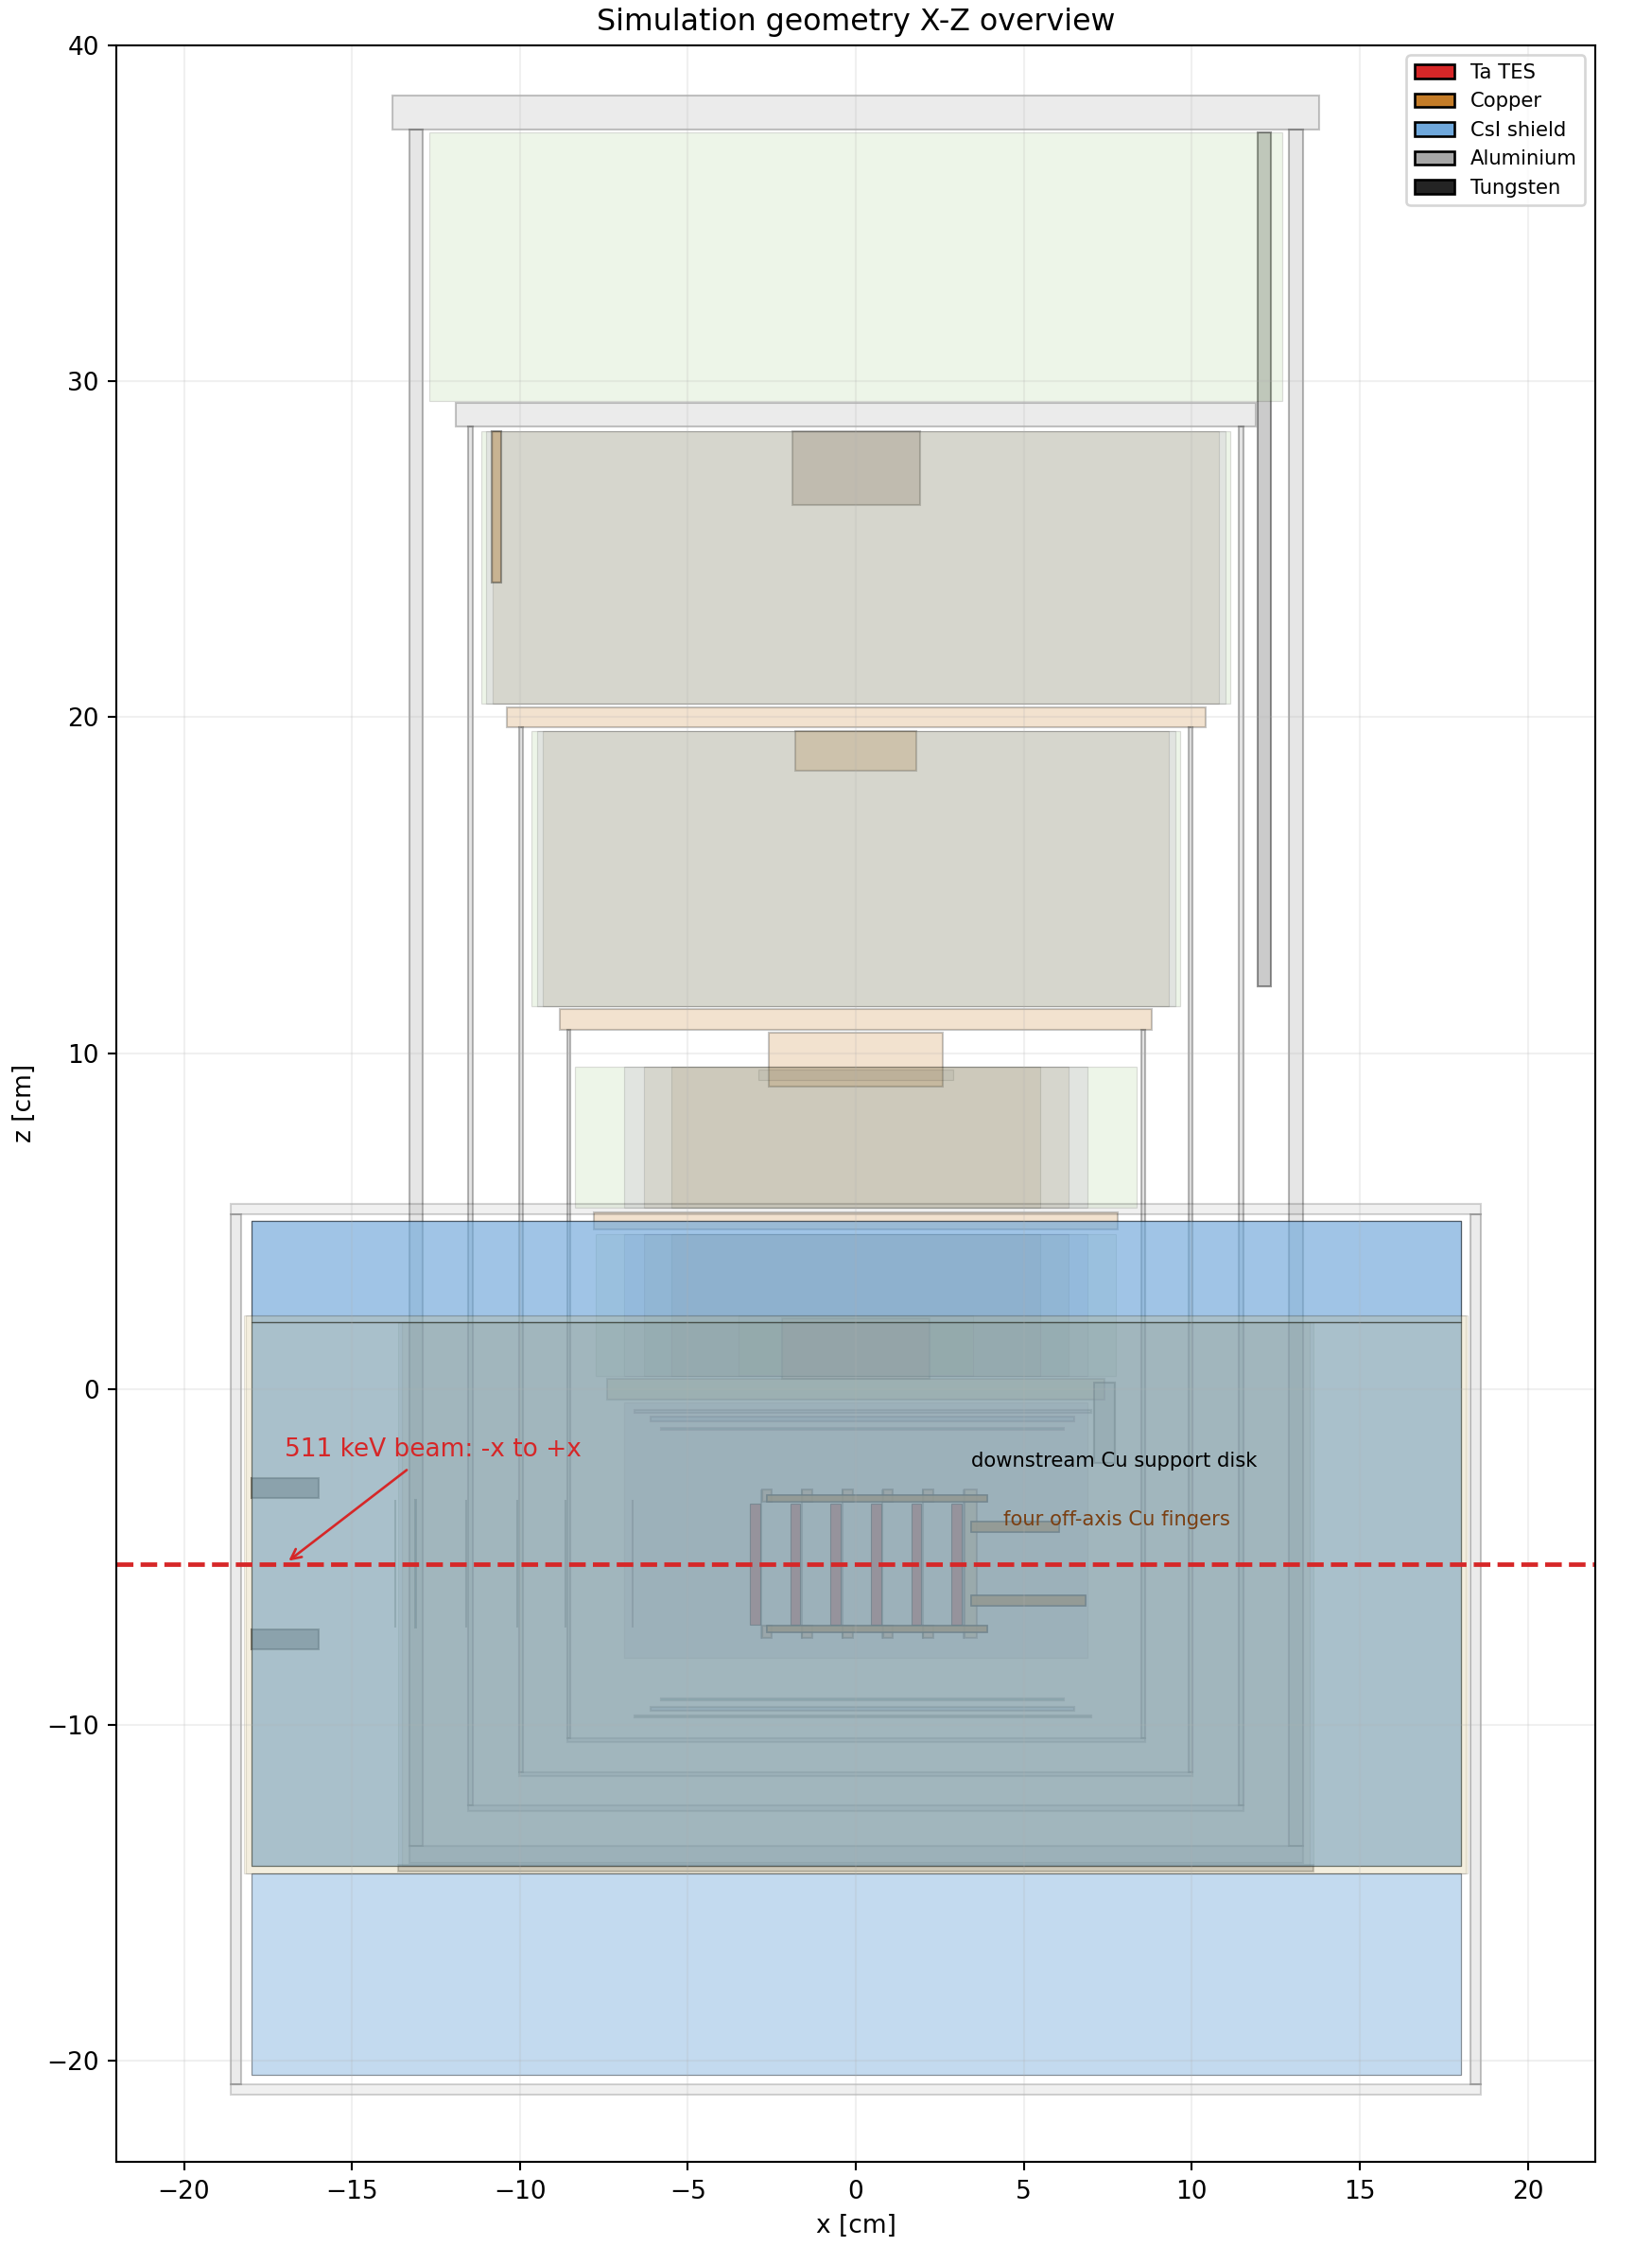
\includegraphics[width=0.62\linewidth]{paper_source_figure_table/fig_mass_model_xz_overview.png}

\vspace{0.6ex}
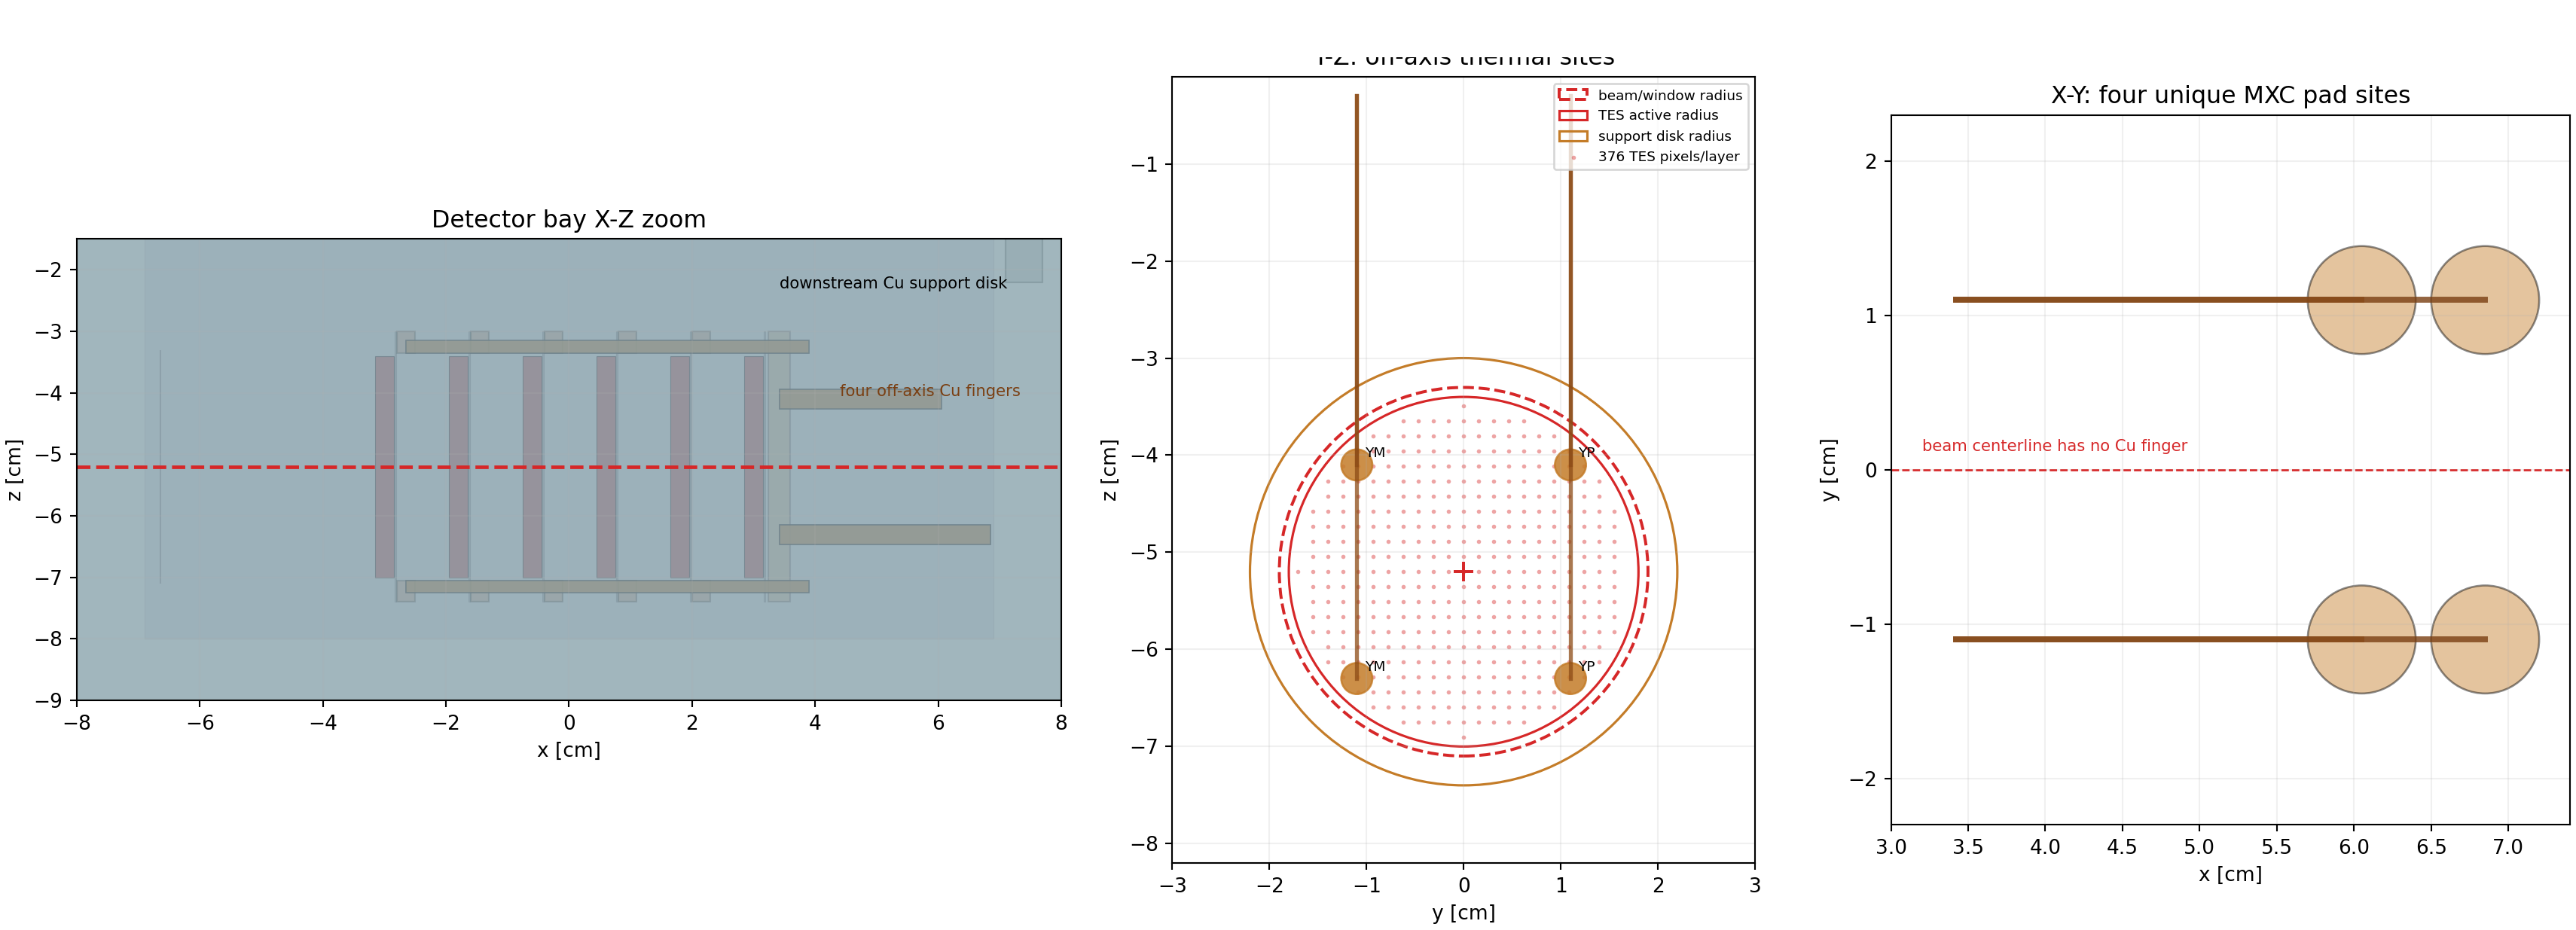
\includegraphics[width=0.88\linewidth]{paper_source_figure_table/fig_mass_model_detector_bay_detail.png}
\caption{基准探测器/低温系统代理质量模型的二维示意图。上：DR 塔、探测器舱、主动屏蔽和 511 keV 侧入射束线的完整 X--Z 视图。下：探测器舱细节，显示 TES 吸收体堆栈、开放中心束区和离轴 Cu 热连接。该图为模拟示意图；x 轴圆形部件和侧孔采用 MEGAlib 兼容代理形状，而不是最终 CAD 实体。}
\label{fig:mass_model}
\end{figure}

\begin{table}[t]
\centering
\caption{主要精确位置链路的探测器与分析参数。}
\label{tab:geometry}
\begin{tabular}{p{0.36\linewidth}p{0.56\linewidth}}
\toprule
参数 & 数值或策略 \\
\midrule
探测器概念 & TES 微量热计焦平面 \\
TES 像素数 & $6\times376=2256$ \\
TES 吸收体代理 & Ta 像素，每个 $1.5\times1.5\times3.0\,\mathrm{mm^3}$ \\
TES 能量响应代理 & 探测器映射中采用 Gaussian $\sigma=0.14\keV$ \\
探测效率处理 & Geant4 输运加后续选后率归一化；此处不强加独立标量效率 \\
主动屏蔽 & 分段 CsI，后处理 veto \\
CsI veto 阈值 & 屏蔽总能量 $50\keV$ \\
入射窗堆栈 & 多级 Al 薄箔和 $150\,\mu\mathrm{m}$ Be 侧窗口 \\
被动屏蔽/准直 & Cu/W 代理衬层、W 底板和 2 cm W 侧套筒 \\
DR/服务质量代理 & MXC/CP/still/4 K/60 K/300 K 温区顺序，以及局部结构、线束和读出服务质量代理 \\
指向 & 局部侧窗口向上倾斜 $45^\circ$ \\
触发/veto 定量定义 & 统一探测器层后处理选择 \\
coincidence 窗 & $1\,\mu\mathrm{s}$ \\
线窗 $\wii$ & $510.58$--$511.42\keV$ \\
参考点源流量 $\fzero$ & $10^{-4}\cms$ \\
\bottomrule
\end{tabular}
\end{table}

\clearpage

\section{Laue 光学与探测器耦合信号重放}
\label{sec:optics}

信号模型采用标准 Laue 透镜思路：入射 $\gamma$ 射线在 mosaic 晶体中以透射 Laue 几何发生 Bragg 衍射，并被集中到小面积焦平面探测器上 \cite{Barriere2009Laue,Barriere2011LauePrototype}。早期聚焦式 $\gamma$ 射线望远镜研究已经指出，探测器响应需要和聚焦相空间一起评估，而不能只用孤立的透镜有效面积代替 \cite{Weidenspointner2006MAX}。针对本文的 511 keV TES 概念 \cite{Shirazi2023}，基准光学构型为单能 Ge(111) Laue 环：焦距 $10\,\mathrm{m}$，25 个方形晶片，晶片边长 18 mm，mosaic FWHM 为 30 arcsec，有效 Ge 质量 $0.44063\,\mathrm{kg}$。Ge(111) 衍射概率和角响应由外部 XOP/CRYSTAL rocking-curve map 给出 \cite{SanchezDelRio2011XOP}。有效面积归一化定义为环几何面积乘以模拟得到的、能够经探测器入口孔径出射的衍射光子比例，得到 $\aeff(511\keV)=20.08476\,\mathrm{cm^2}$。

光学模拟在本文中作为聚焦信号源生成器，而不只是一个孤立有效面积计算。在输运过程中，穿过标称焦面的 $\gamma$ 光子会连同其能量、位置、方向和产生历史一起记录。只有经过真实追踪、发生 Laue 衍射并落入 Be 入射孔径的光子才传递给后续探测器模拟；解析光斑投影只作为诊断量保留。这样保留了衍射光子离开 Ge 晶体时的吸收和散射效应。

图~\ref{fig:optics_transport_schematic} 和图~\ref{fig:optics_focal_spot} 分别给出光学-探测器耦合的两个层次：由 Laue 环配置到焦面的径向光学约束，以及注入探测器模型的横向分布。

\begin{figure}[t]
\centering
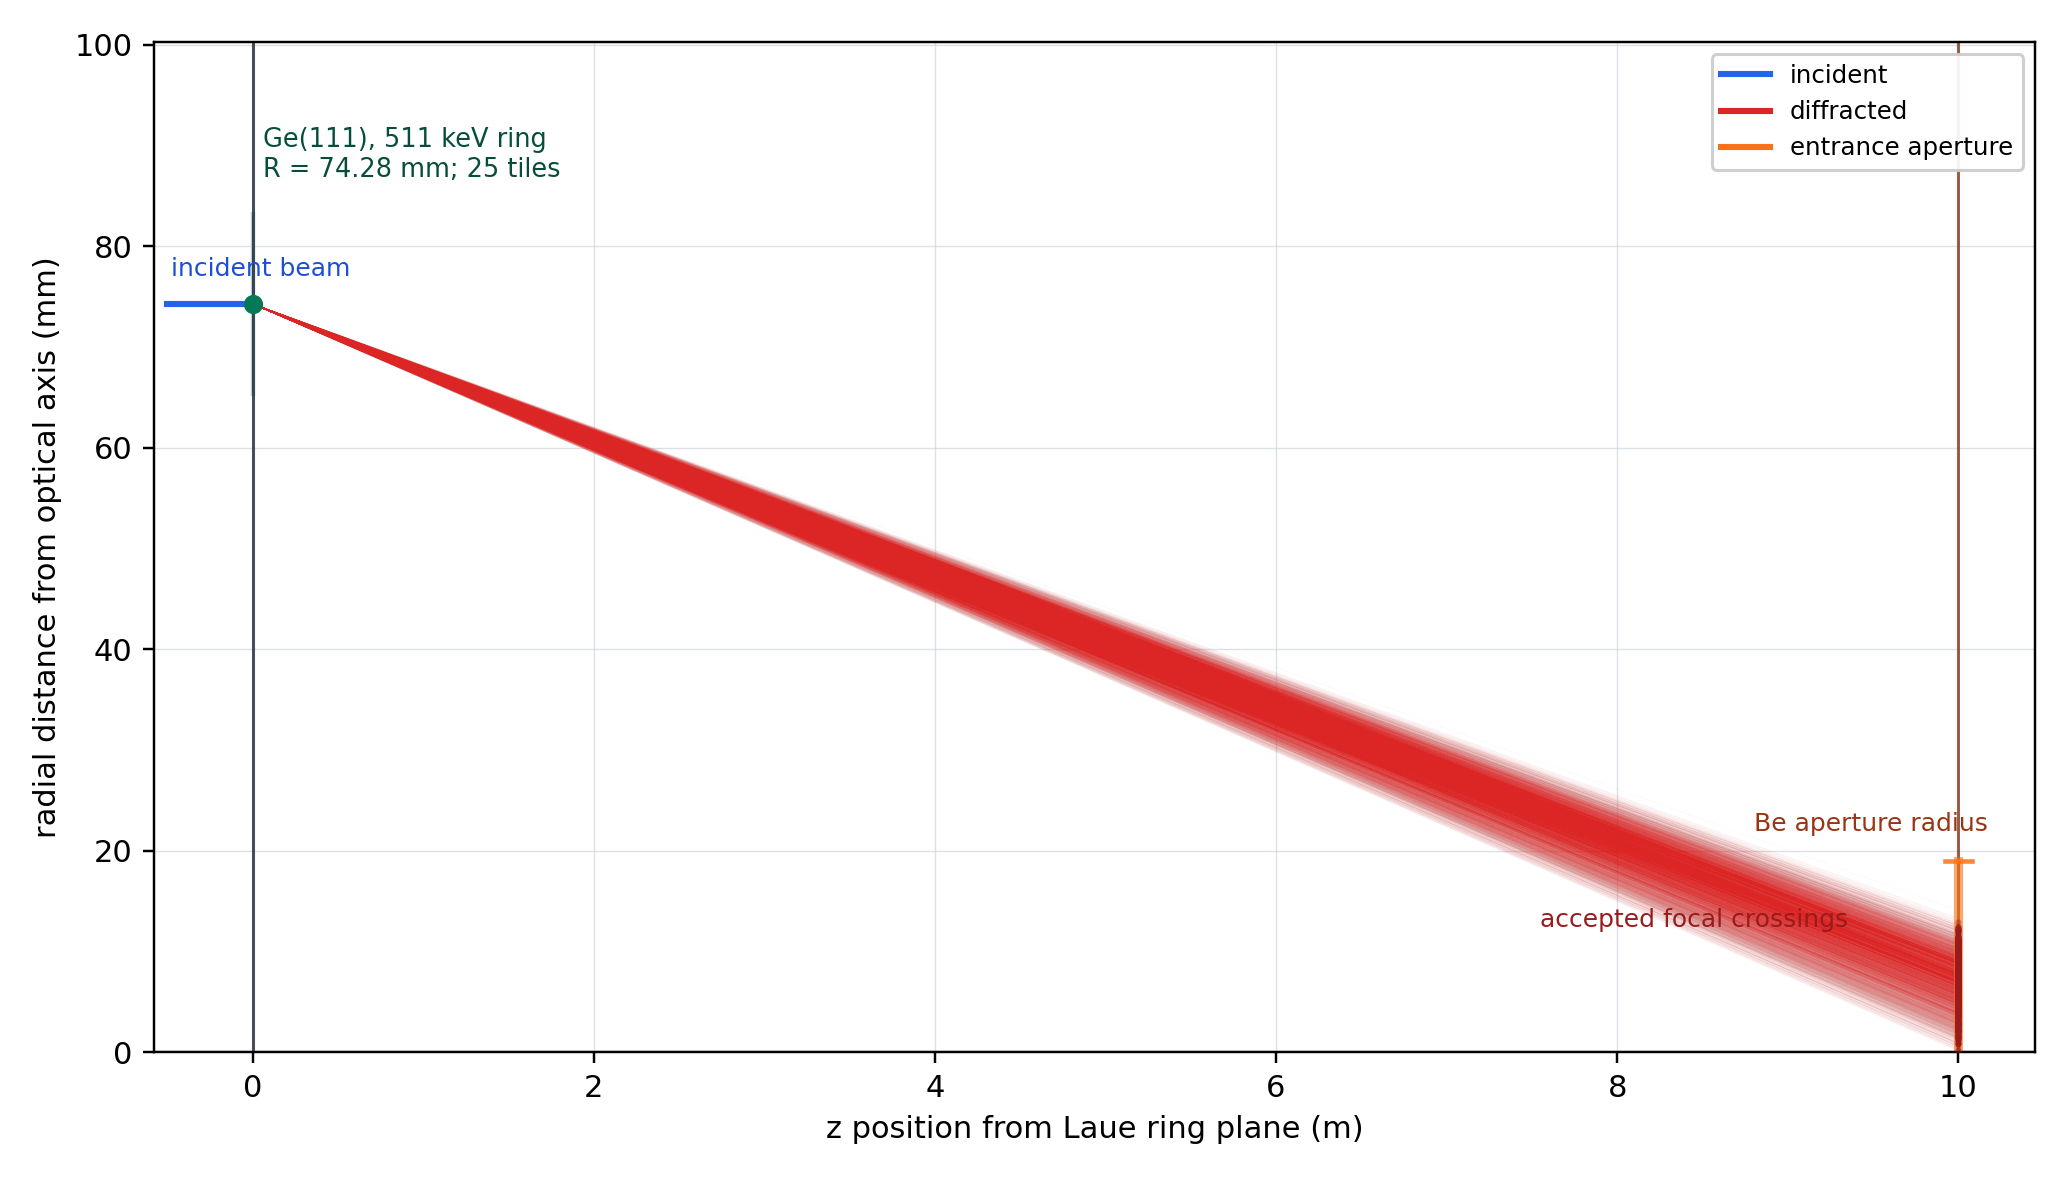
\includegraphics[width=0.96\linewidth]{paper_source_figure_table/fig_optics_laue_transport_schematic.png}
\caption{基准 511 keV Laue 信号源的数据约束径向--$z$ 可视化。Laue 平面、Ge(111) 环半径和晶片足迹、$10\,\mathrm{m}$ 焦距以及 Be 入射孔径半径均来自当前光学配置。红色衍射扇束终止于真实追踪且通过入射孔径筛选的焦面穿越点。该图压缩了方位角晶片排布，只用于说明由输运输出支撑的探测器输入。}
\label{fig:optics_transport_schematic}
\end{figure}

\begin{figure}[t]
\centering
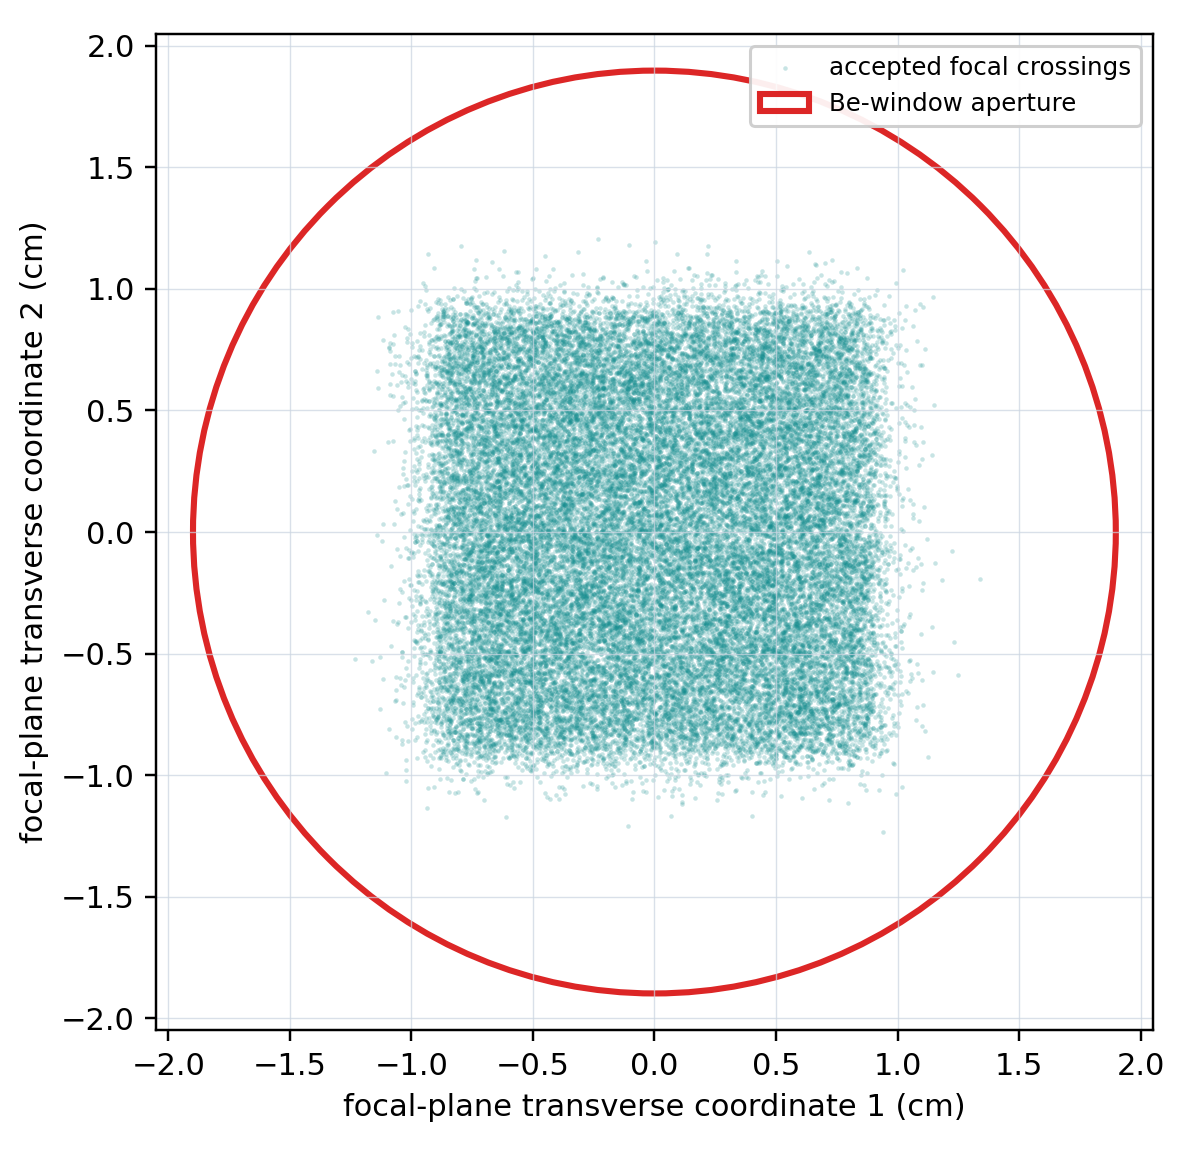
\includegraphics[width=0.58\linewidth]{paper_source_figure_table/fig_optics_focal_crossings_xy.png}
\caption{通过 Be 入射孔径筛选、并用于后续探测器重放的真实追踪焦面横向位置。红色圆为 Be 窗孔径。该分布是探测器输入平面上的输运光学相空间，而不是解析光斑投影。}
\label{fig:optics_focal_spot}
\end{figure}

通过 Be 入射孔径的焦面光子被转换到局部侧入射探测器坐标系，并在探测器/低温系统质量模型中重放。这样保留了探测器入口平面的模拟位置和方向分布，避免用解析光斑替代光学计算。因此，这里的焦面穿越表是输运得到的光学信号输入：它记录 511 keV 源模拟中穿过焦面的 $\gamma$ 光子，而不是由大气或宇宙线与上游透镜硬件相互作用产生的粒子。

为了检验这一边界能否在需要时由同一 Geant4/MEGAlib 本底链处理，本文还运行了一个辅助的上游硬件计算。该计算在 10 m 上游透镜位置放置一个与 Laue 有效晶体等体积、等质量的 Ge 代理体。该代理体对应 25 个方形 Ge 晶片，边长 18 mm、厚度 10.218801 mm，总有效 Ge 体积为 $82.7723\,\mathrm{cm^3}$，质量为 $0.4406\,\mathrm{kg}$。大气远场源面不再沿用局部探测器的 60 cm 源球，而是由探测器加上游透镜的组合包络确定：10 m 透镜中心距离加有效晶体体积包络给出 $1008.8\,\mathrm{cm}$，输运源面半径向上取整为 $1060\,\mathrm{cm}$，世界体半尺寸为 $2500\,\mathrm{cm}$。在低统计量接口测试之后，该质量代理又使用与探测器本底链相同的八类 EXPACS/PARMA 粒子族（$\gamma$、$n$、$e^\pm$、$p$、$\alpha$ 和 $\mu^\pm$）完成了生产级瞬发输运和活化产生输运。该计算定义了上游质量代理的全粒子输运和同位素产生边界。有效 Ge 代理体产生的延迟成分随后从组合几何同位素清单中隔离出来，并按记录产生位置转换为衰变源，在同一探测器层选择下重放；其选后率结果在第~\ref{subsec:upstream_optics_background} 节给出。

对于聚焦点源响应，$\fzero=10^{-4}\cms$ 是用于归一化的入射 511 keV 光子流量。硬线窗信号响应 $0.00118587\cps$ 指该流量下经过探测器输运、参考大气透过因子和探测器层事例选择后的 $\wii$ 信号计数率。源流量响应是相应的线性系数，$S_{\wii}/\fzero=11.8587\,\mathrm{s^{-1}}/(\mathrm{ph\,cm^{-2}\,s^{-1}})$。该参考归一化应理解为基准指向情形，而不是所有气球指向通用的大气透过率。低仰角或长斜程观测，包括北半球中纬度气球轨迹上的银河中心观测，应使用斜程大气透过模型；这类斜程计算仍是边界检查，不替代当前硬线窗头条结果。

\section{瞬发大气与延迟活化源模型}
\label{sec:background}

\subsection{瞬发大气源}
\label{subsec:prompt_source}

本底源模型被分为瞬发大气输运和延迟活化两条线，以避免把源产生过程和探测器选择假设混在一起。瞬发大气粒子场由 EXPACS/PARMA 给出。PARMA3.0 是由 PHITS 大气级联计算参数化得到、并针对陆地宇宙线场验证的解析模型，EXPACS 是其公开表格/软件接口 \cite{Sato2015EXPACS}。PHITS 提供其底层粒子输运物理：一次宇宙线与大气核相互作用，产生的次级强子、轻子、光子和中子在大气柱中继续输运，最终通量再按海拔、地磁截止刚度、太阳调制、能量和方向参数化。在本文中，EXPACS/PARMA 给出随粒子种类、动能、天顶角、地理位置、海拔、地磁截止刚度和太阳调制变化的入射微分通量。它只用于构造外部辐射场；探测器响应、反符合、拓扑选择和任务时间计数均在后续步骤施加。本文参考源定义采用纬度 $34^\circ$、经度 $100^\circ$、海拔 $38\,\mathrm{km}$、垂直截止刚度 $R_c=11.6\,\mathrm{GV}$，以及 2025-08-31 对应的太阳调制条件 $W=118.3$。

瞬发源包含光子、中子、电子、正电子、质子、$\alpha$ 粒子、负 $\mu$ 子和正 $\mu$ 子。对每个粒子族，EXPACS/PARMA 微分谱被转换为 MEGAlib 远场面积源，覆盖完整天顶角范围 $\theta=0^\circ$--$180^\circ$ 和完整方位角范围 $\phi=0^\circ$--$360^\circ$。天顶角依赖用 20 个等 $\mu$ 微分角度分箱表示，其中 $\mu=\cos\theta$，每个分箱的立体角为 $\Delta\Omega=0.6283185307\,\mathrm{sr}$。前 10 个分箱表示下行粒子（$0^\circ\leq\theta\leq90^\circ$），后 10 个分箱表示上行或反照成分（$90^\circ\leq\theta\leq180^\circ$）。瞬发输运和活化产生输运都保留这两个半球，因此源构建阶段没有丢弃上行反照粒子。

图~\ref{fig:expacs_fullsphere_flux} 给出由源定义实际采用的全空间通量场。

\begin{figure}[t]
\centering
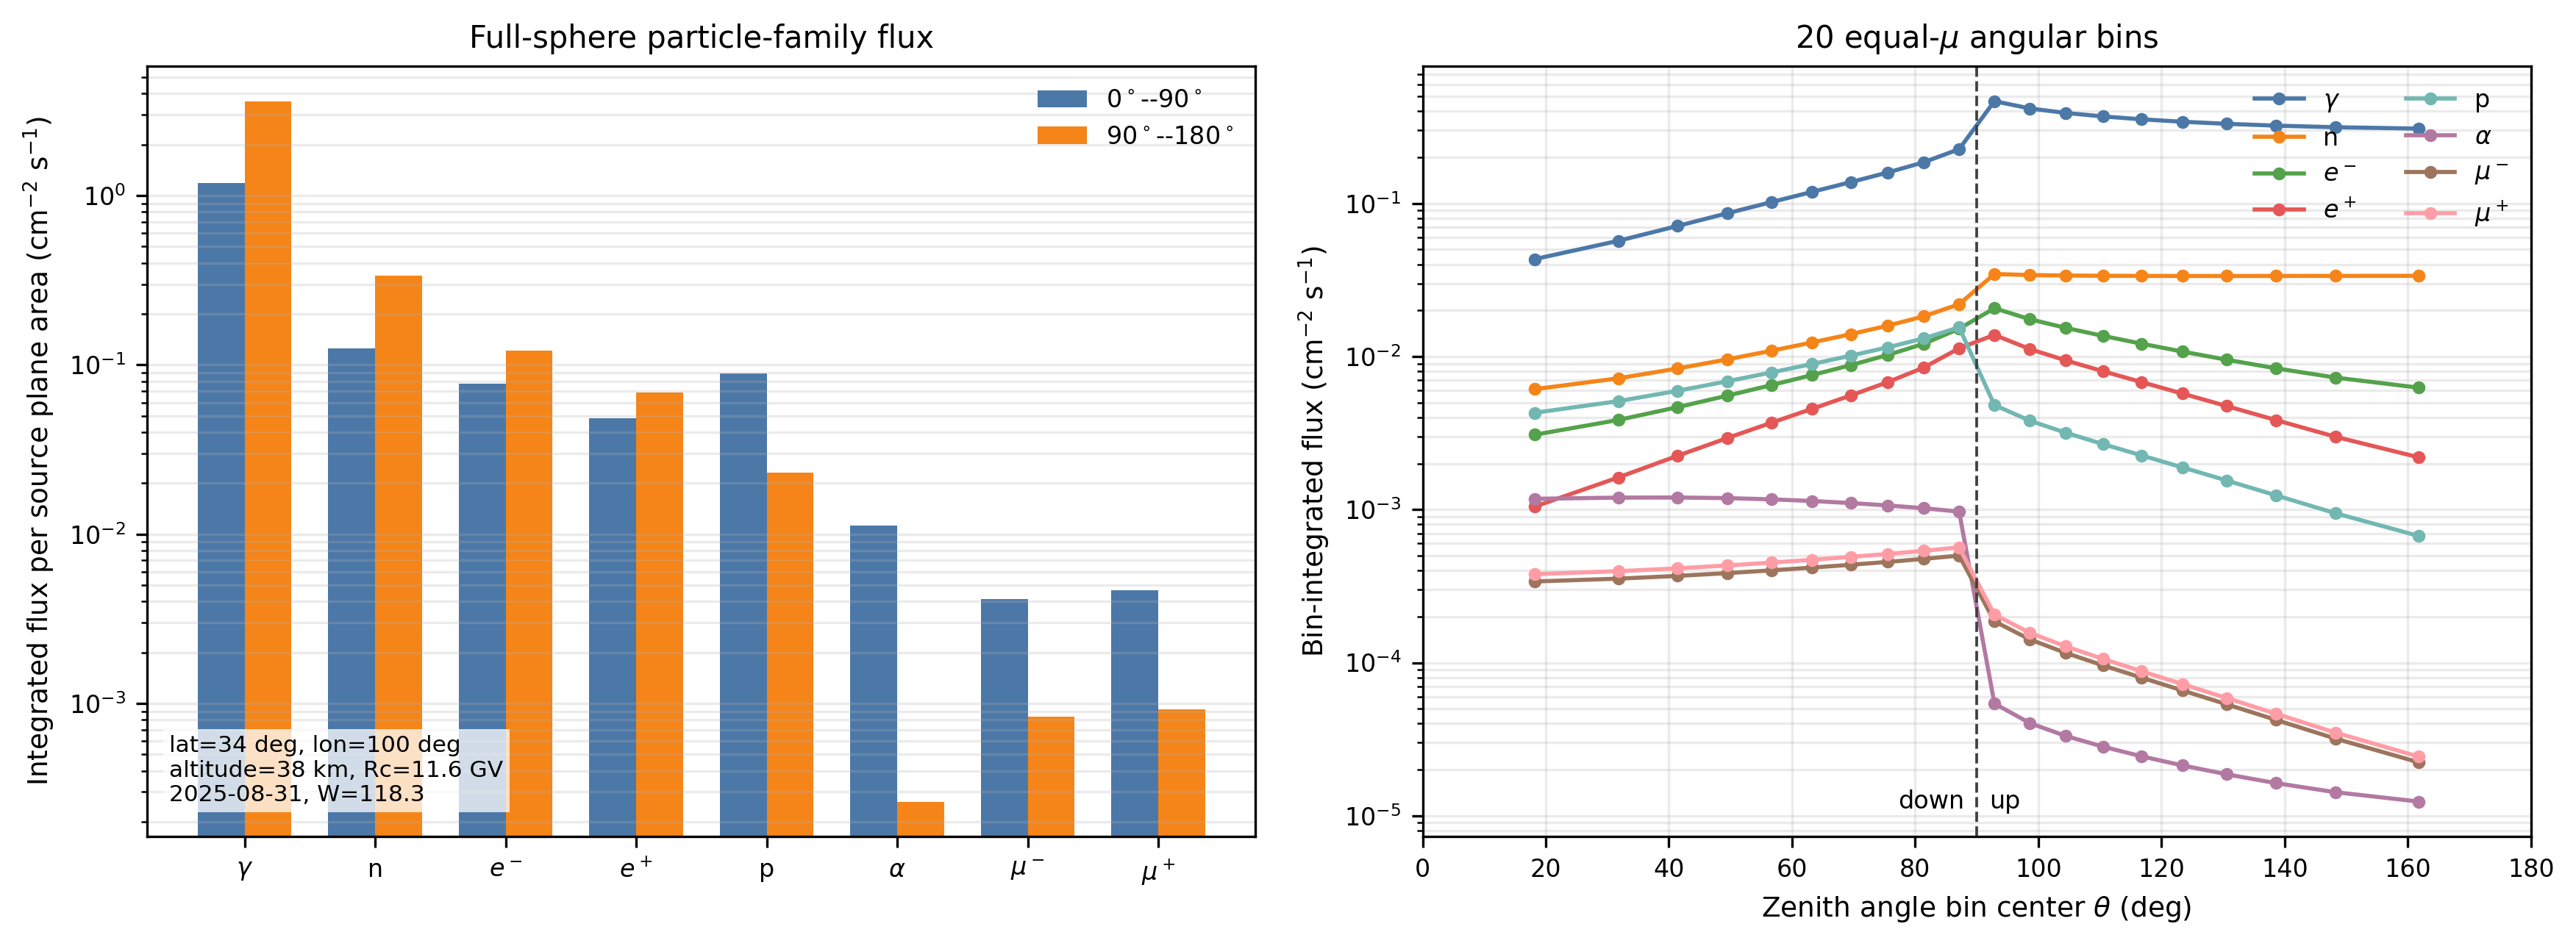
\includegraphics[width=\linewidth]{paper_source_figure_table/fig_expacs_fullsphere_flux.png}
\caption{用于生成瞬发和活化产生输运输入的 EXPACS/PARMA 全空间大气通量场。左：八类输运粒子族的能量和立体角积分通量，并按下行、上行半球分开。右：MEGAlib 远场源使用的 20 个等 $\mu$ 微分天顶角分箱的积分通量。该图直接由源定义输入表生成，环境参数为纬度 $34^\circ$、经度 $100^\circ$、海拔 $38\,\mathrm{km}$、$R_c=11.6\,\mathrm{GV}$、$W=118.3$。}
\label{fig:expacs_fullsphere_flux}
\end{figure}

其中主导成分为 $\gamma$、$n$、$e^-$、$e^+$ 和 $p$，源面积分通量分别为 $4.79966$、$0.462239$、$0.199002$、$0.116981$ 和 $0.112301\,\mathrm{cm^{-2}\,s^{-1}}$；$\alpha$、$\mu^-$ 和 $\mu^+$ 成分低一个到数个量级，但仍保留在输运输入中。非光子成分合计约为 $0.913\,\mathrm{cm^{-2}\,s^{-1}}$，约占全空间源面积分通量的 16\%。如果完全按流量比例分配模拟计数，这些低通量粒子的探测器命中和活化统计会较差；因此非光子粒子族采用复制输运样本提高 Monte Carlo 统计，再在率归一化时去权重。所有这些粒子随后通过 Geant4/MEGAlib 在探测器/低温系统质量模型中输运 \cite{Agostinelli2003,Zoglauer2006}。瞬发流和活化产生流各生成 25,210,216 个入射一次粒子。每个粒子种类用自身输运曝光归一化：
\begin{equation}
  r_{\mathrm{event},j}=\left(\sum_i \mathcal{T}_{ij}\right)^{-1},
\end{equation}
其中 $\mathcal{T}_{ij}$ 为第 $j$ 个粒子种类在第 $i$ 个输运子样本中的曝光。由于光子和非光子大气流的采样与曝光结构不同，这种按粒子种类归一化是必要的。归一化检查要求每个粒子种类满足 $r_{\mathrm{event},j}\sum_i\mathcal{T}_{ij}=1$，因此过采样只改变 Monte Carlo 方差，不改变物理期望率。

\subsection{延迟活化源}
\label{subsec:delayed_source}

活化产生流不作为瞬时探测器本底直接计数，而是记录放射性产物的核素、材料体积和产生位置。这些记录通过产生--衰变积累方程转换为固定第 15 天放射性群体，并使用 NUBASE2020 校验过的基态半衰期修正 \cite{Kondev2021NUBASE}。对核素 $k$，
\begin{equation}
  A_k(t_{\mathrm{flight}}) = R_k\left[1-\exp\left(-\lambda_k t_{\mathrm{flight}}\right)\right],
  \qquad \lambda_k = \frac{\ln 2}{t_{1/2,k}},
\end{equation}
其中 $R_k$ 是由活化产生输运推得的产生率，参考清单取 $t_{\mathrm{flight}}=15\,\mathrm{d}$。当前 fix5 链路使用的固定延迟总活度为 $85.449203\,\mathrm{Bq}$。

位置信息并不是只来自聚合后的同位素存储文件。标准同位素存储可记录产生体积和核素计数；精确位置链路还在 Geant4/MEGAlib 的 stepping-action 层加入了自定义记录钩子。在活化积累模式中，每当一个延迟核素被存入同位素清单时，该钩子在同一位置写出产生位置记录，包括逻辑体名称、pre-step 位置 $(x,y,z)$、核素编号 $1000Z+A$、激发能、时间、过程以及 track ancestry 信息。固定第 15 天放射性群体随后按体积、核素和激发态与这些位置记录匹配。因此，延迟源使用的是真实模拟产生坐标，而不是只有体积积分活度。

图~\ref{fig:delayed_exactpos_distribution} 给出放射性产生位置与固定第 15 天活度群体匹配后的延迟源位置分布。

\begin{figure}[t]
\centering
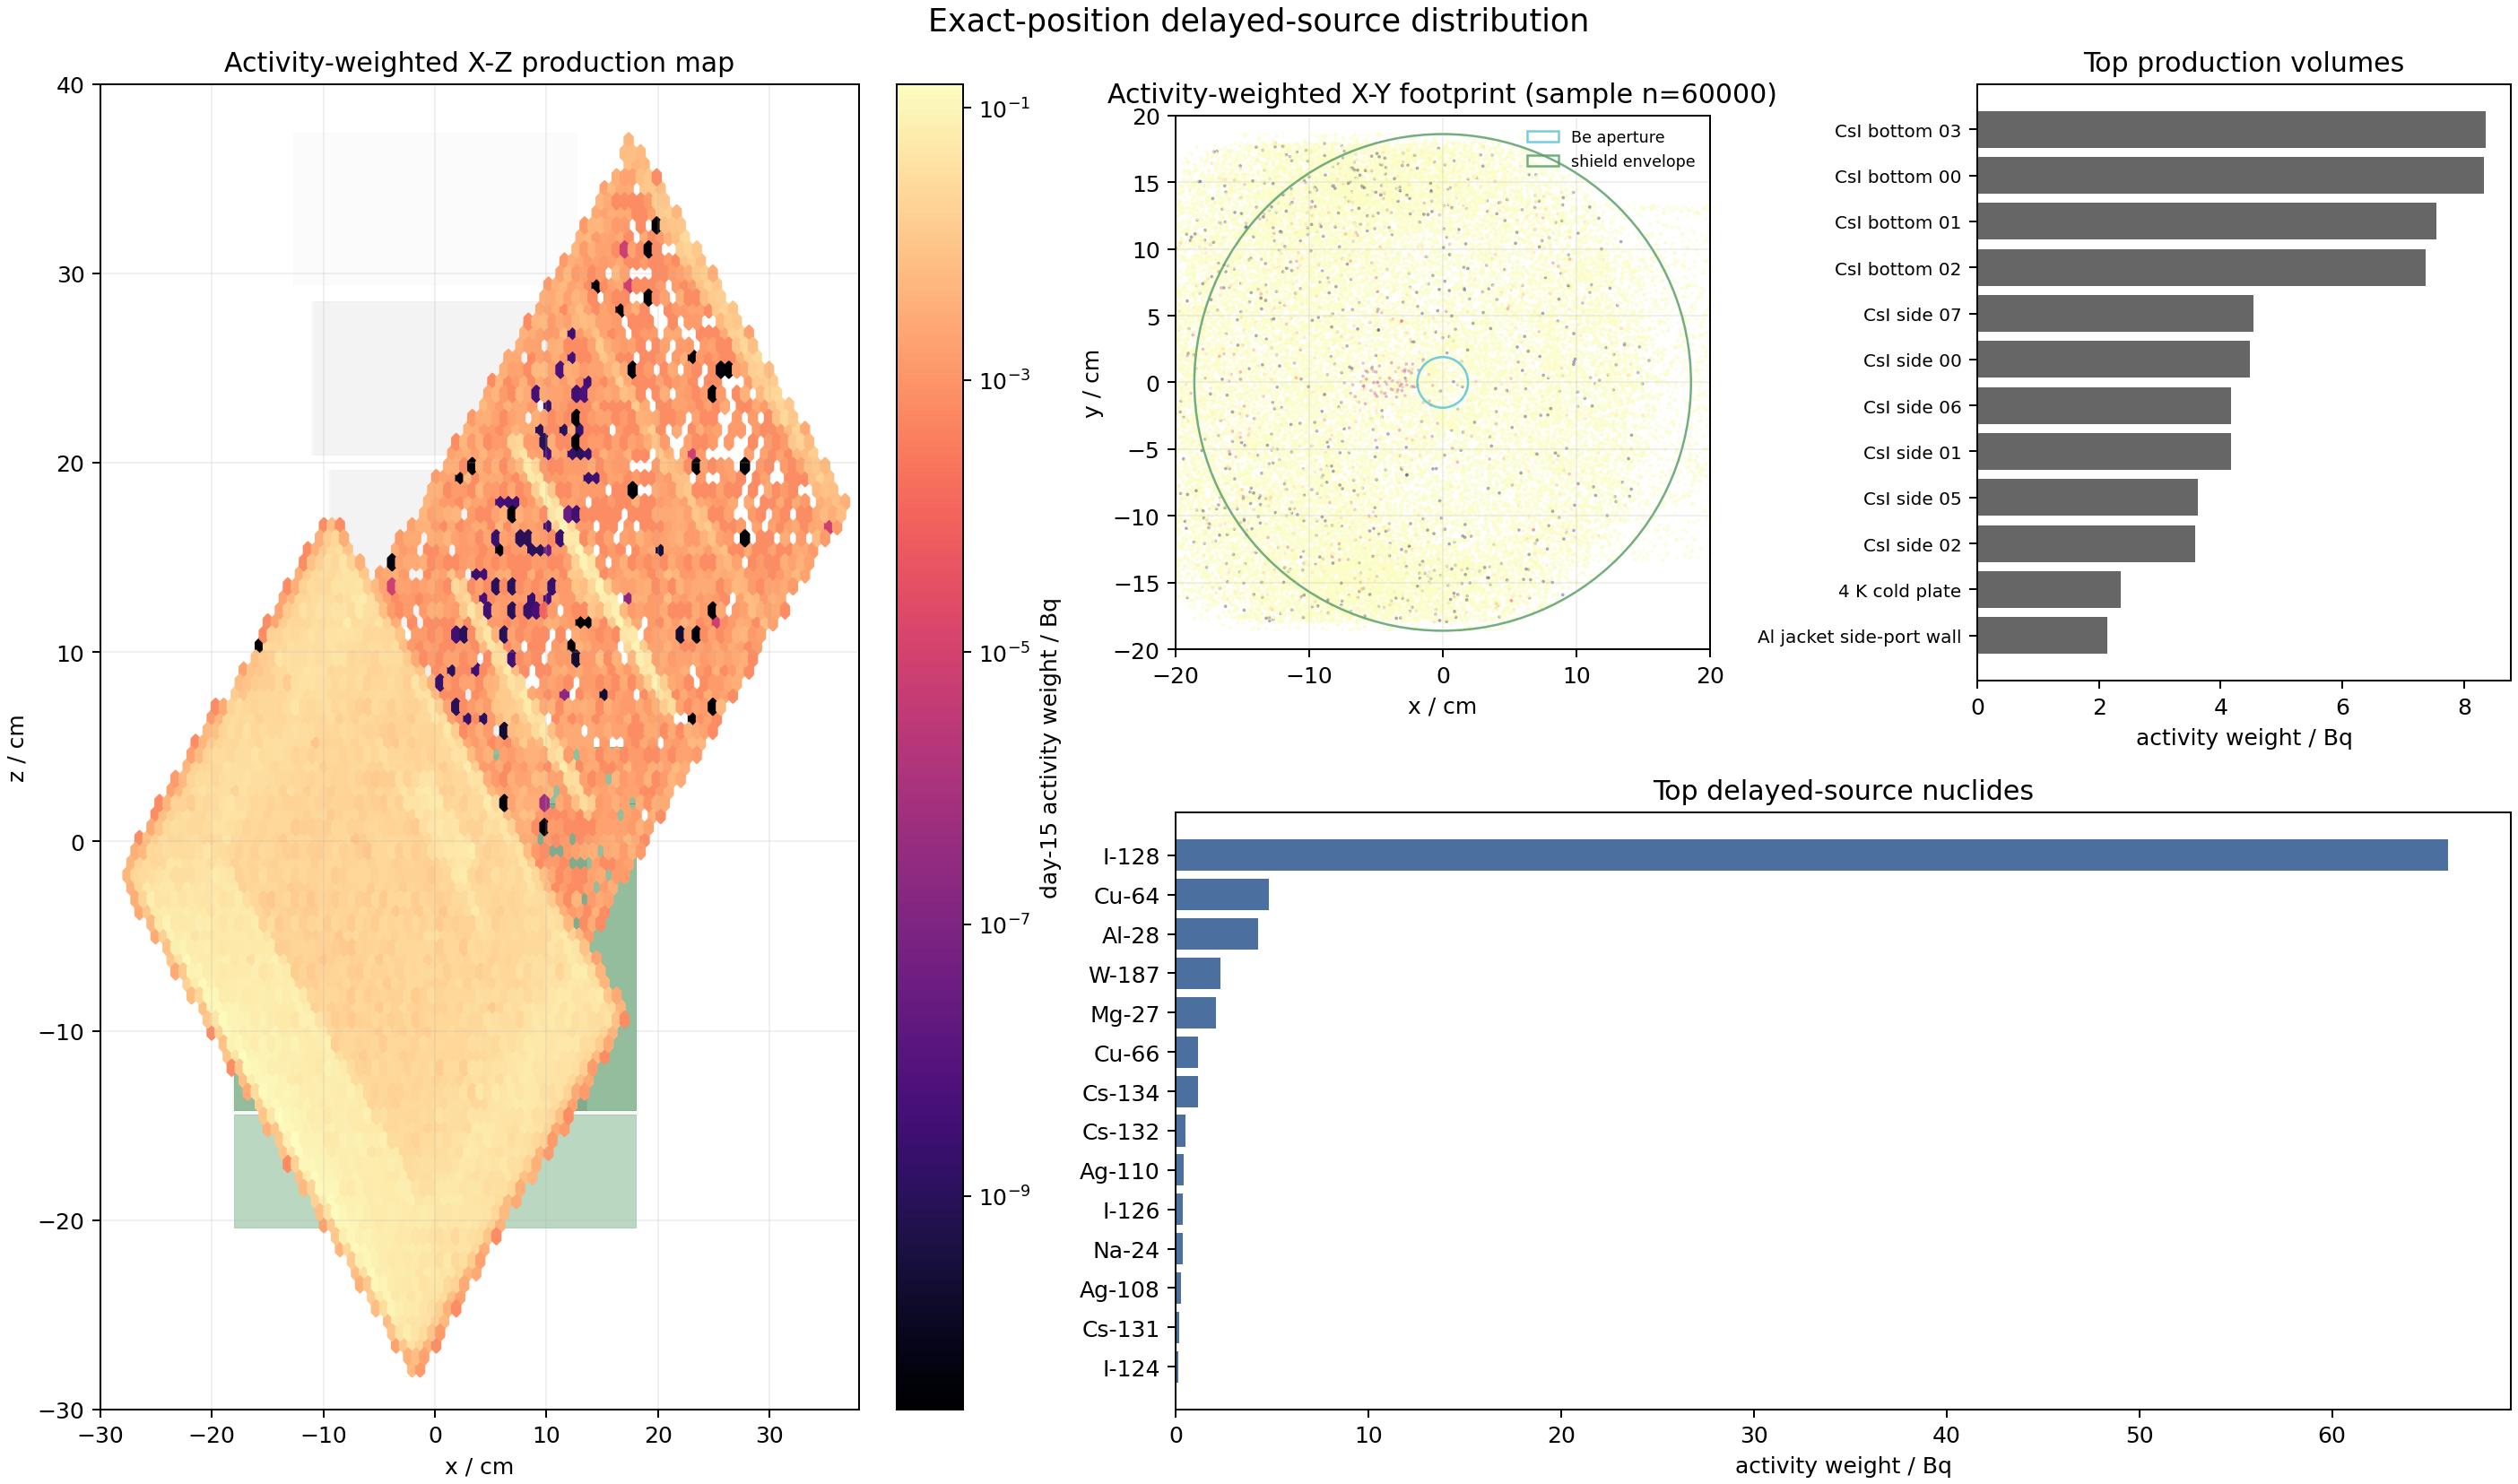
\includegraphics[width=\linewidth]{paper_source_figure_table/fig_delayed_exactpos_rpip_distribution.png}
\caption{由当前 fix5 链路真实放射性核素产生位置构建的精确位置延迟源样本。左：记录产生位置在 X--Z 平面上的活度加权分布，并叠加探测器/低温系统代理几何。中上：同一分布的 X--Y 活度加权足迹，图中给出 Be 孔径和屏蔽包络作为尺度参考。右侧和下方：按固定第 15 天活度加权后的主要产生体积和主要核素。匹配后的产生位置表中活度权重总和为 $85.449203\,\mathrm{Bq}$。}
\label{fig:delayed_exactpos_distribution}
\end{figure}

活度加权分布主要来自 CsI 主动屏蔽活化和 $^{128}$I，较小贡献来自 Cu、Al、W、Mg 和 Cs 等核素。该图是源构建诊断图，不是探测器计数图；探测器响应只有在延迟衰变通过同一几何和同一事例选择输运后才施加。

是否需要精确位置抽样，也可以直接用同一张产生位置表检验。延迟衰变是在局部材料中发射的，因此下游衰减、主动屏蔽 veto 概率和事例拓扑都取决于核素产生位置。带电强子和缪子相对中子有不同的能量损失、停止和俘获历史，因此它们产生的活化核素不应被假定为共享同一个材料或坐标分布。为量化这一点，我们按入射粒子族和材料类别对加权产生行分组。对两个入射粒子族 $a$ 和 $b$，使用活度归一化材料分布的 total-variation 距离
\begin{equation}
  D_{\mathrm{TV}}(a,b) =
  \frac{1}{2}\sum_c \left| f_{a,c} - f_{b,c} \right| ,
\end{equation}
其中 $f_{a,c}$ 为入射粒子族 $a$ 在材料类别 $c$ 中产生的延迟活度占比。

图~\ref{fig:exactpos_sampling_necessity} 给出这一检验结果。

\begin{figure}[t]
\centering
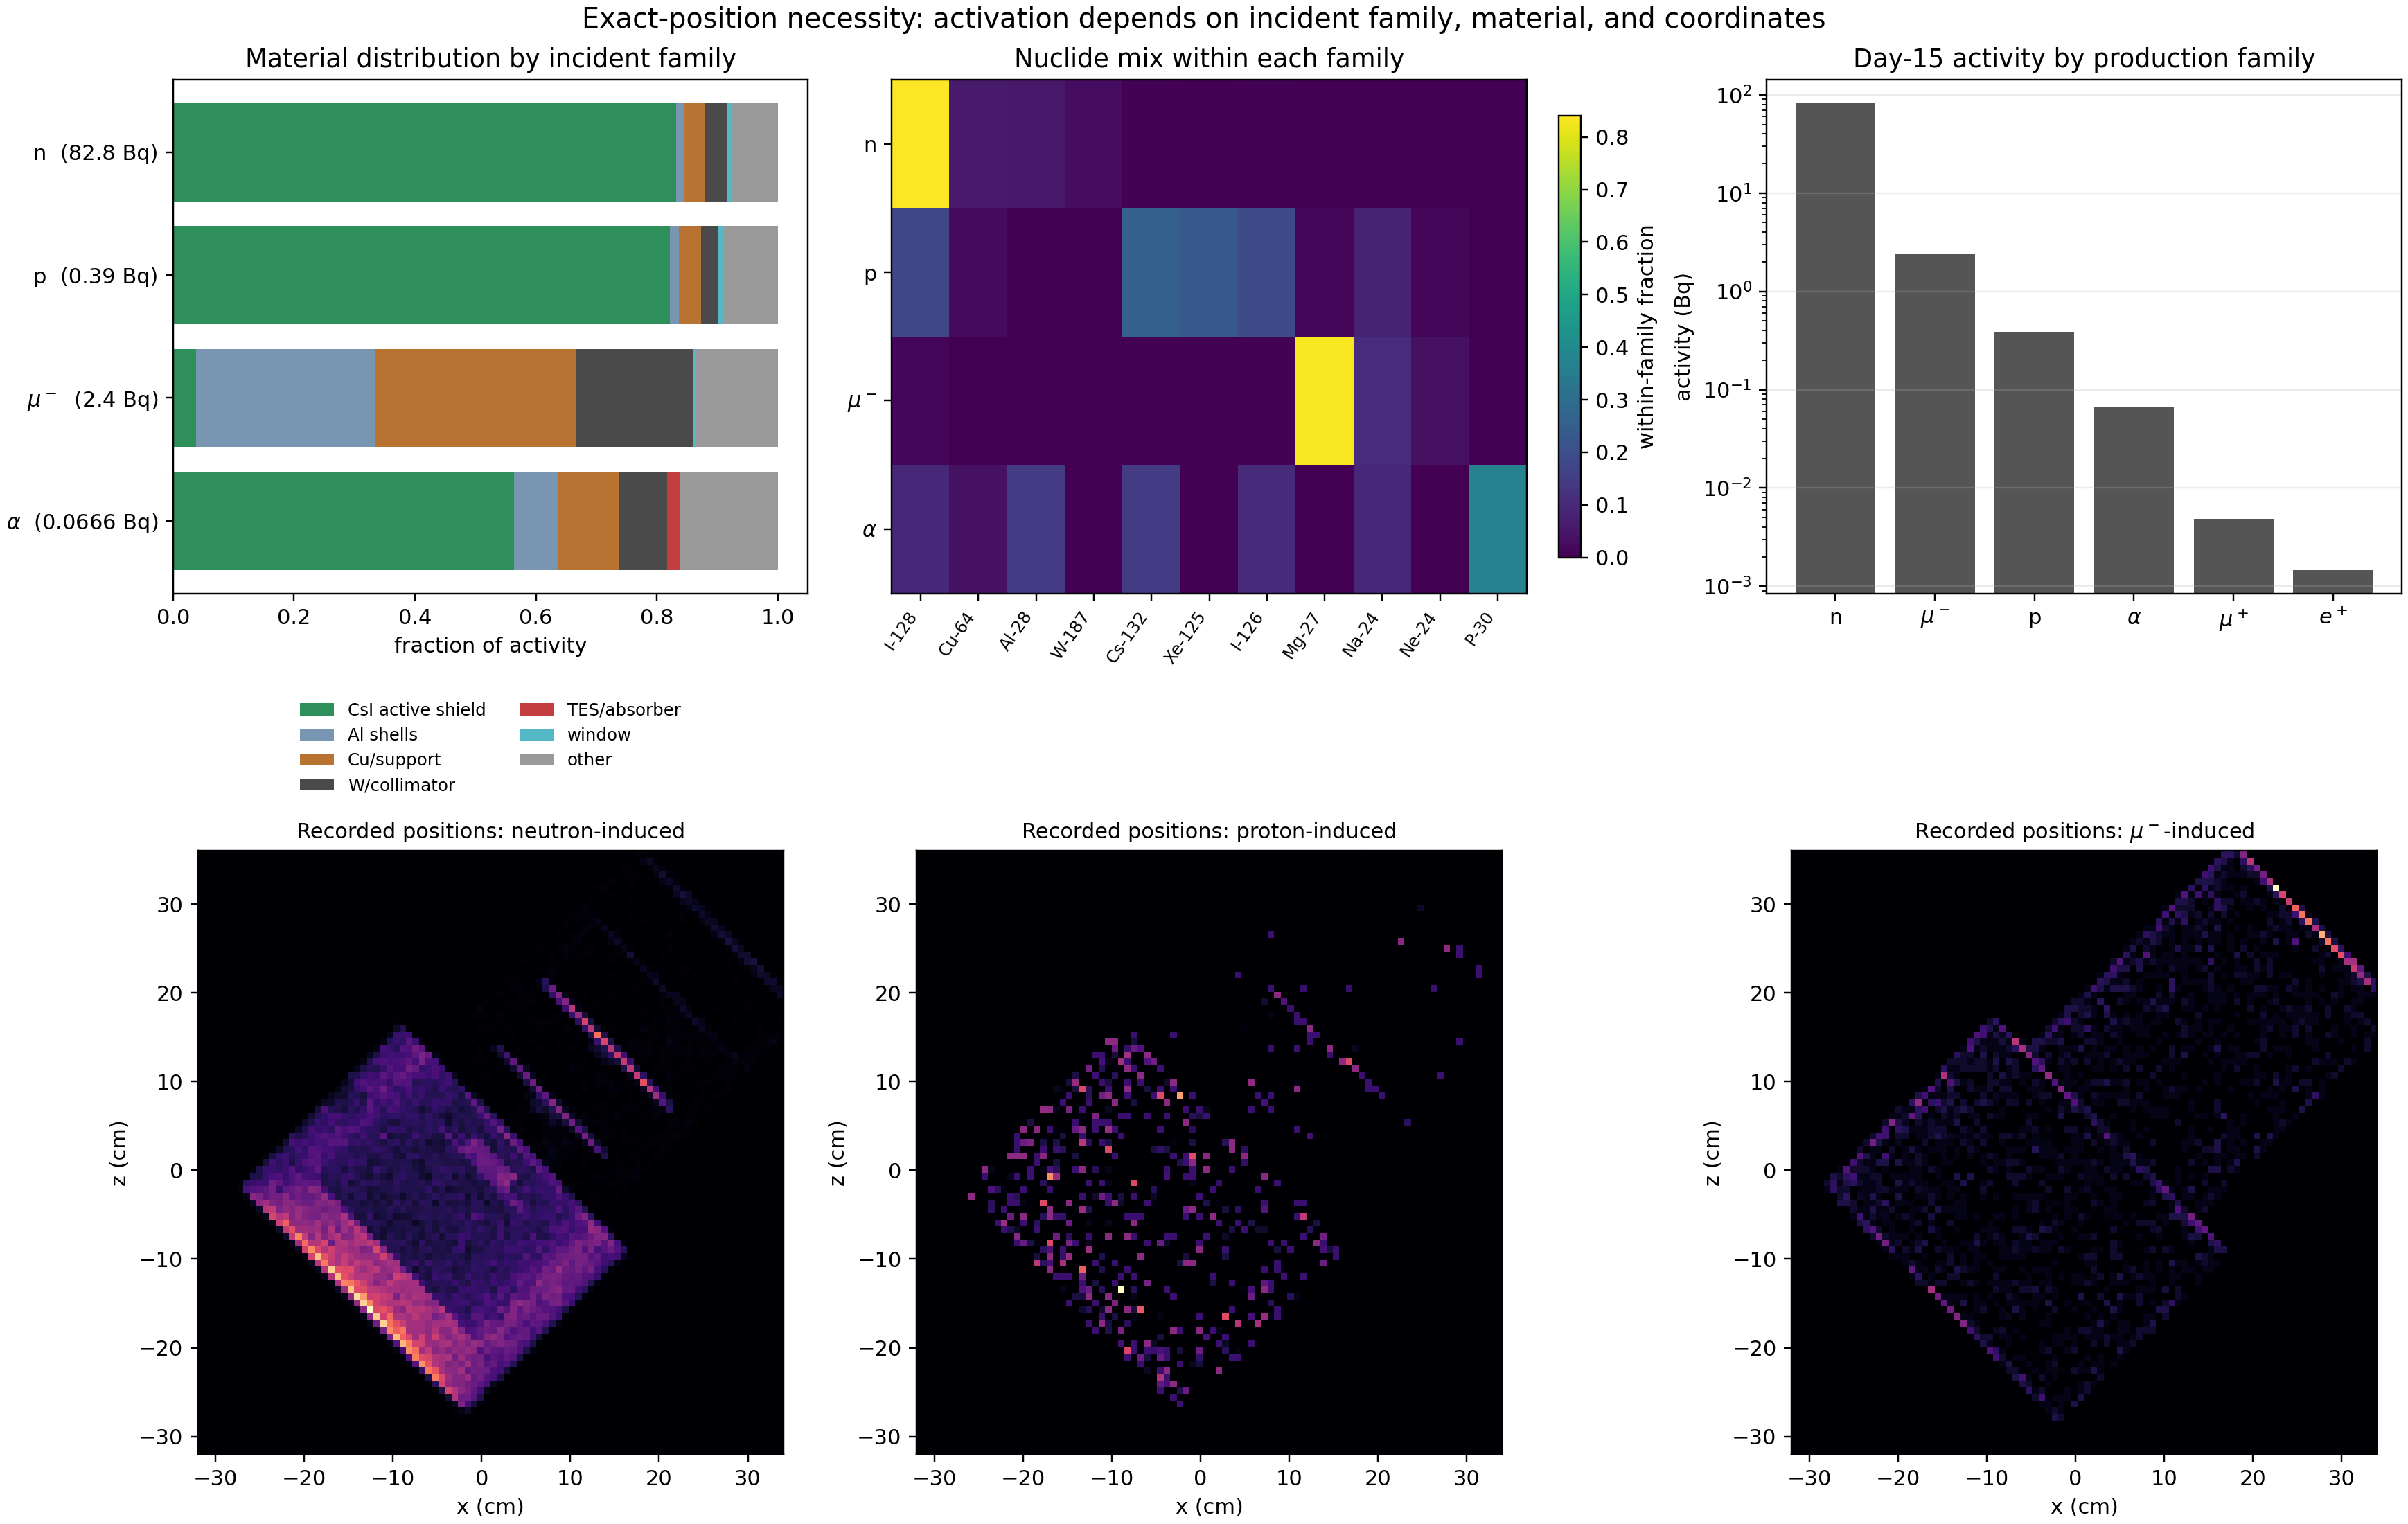
\includegraphics[width=\linewidth]{paper_source_figure_table/fig_exactpos_sampling_necessity.png}
\caption{精确位置延迟源抽样必要性的真实数据检验。上排按入射粒子族比较固定第 15 天加权产生表：材料占比、核素组成和总活度。下排给出中子、质子和 $\mu^-$ 诱发产物的 X--Z 真实产生位置图。不同入射粒子族的分布并不可互换：中子诱发活度主要在 CsI 和 $^{128}$I 中，$\mu^-$ 诱发活度则集中在 Al/Cu/W 服务和屏蔽质量中，并以 Mg/Na/Ne 产物为主。}
\label{fig:exactpos_sampling_necessity}
\end{figure}

在固定第 15 天表中，中子诱发产物贡献 $82.522\,\mathrm{Bq}$，$\mu^-$ 诱发产物贡献 $2.752\,\mathrm{Bq}$，质子诱发产物贡献 $0.147\,\mathrm{Bq}$，$\alpha$ 诱发产物贡献 $0.0223\,\mathrm{Bq}$，另有更小的 $\mu^+$ 和 $e^+$ 贡献。中子诱发活度仍主要产生在 CsI 主动屏蔽中；$\mu^-$ 成分则明显不同，其中 Cu/支撑材料、Al 壳层和 W/准直器材料分别占 $\mu^-$ 诱发活度的 32.2\%、28.5\% 和 20.5\%。固定源中 W/准直器体积活度为 $0.986\,\mathrm{Bq}$，占固定延迟活度的 1.154\%。由于选后事例审计在硬线窗样本中找到零个 W/准直器来源延迟选后事例，这个源级 W 活化没有成为主导的选后率成分。因此，体积积分源或轴对称径向源可以保持总活度，但会抹掉入射粒子族、材料、核素和坐标之间的相关性。精确位置构造在进入探测器输运之前保留了这些相关性。

延迟衰变源随后从采样的产生位置发射，而不是从轴对称径向分布发射。设加权产生表中第 $j$ 行的活度权重为 $w_j$，总活度为 $A=\sum_j w_j$。精确位置近似以 $p_j=w_j/A$ 为概率有放回抽取 $M$ 个产生位置，并给每个采样点源相同通量 $A/M$。因此第 $j$ 行获得的期望活度为
\begin{equation}
  \mathbb{E}\!\left[N_j\frac{A}{M}\right] = M p_j \frac{A}{M} = w_j ,
\end{equation}
所以该估计保持总活度，并且对加权空间分布无偏。这里的 $M$ 表示用于近似加权产生位置分布的等活度点源采样点数；它是采样规模，不是物理放射性产生行的数量。用于当前 fix5 主要率级结果的源从完整加权产生表中抽取 $M=50000$ 个点源采样点，随机种子为 260613。这些采样点在源定义层面精确保持总固定活度，并在与瞬发流相同的探测器/低温系统几何中重放。主要 fix5 延迟计算输运 $10^6$ 个延迟衰变，Cosima live time 为 $11649.564832\,\mathrm{s}$。该 live time 是生成衰变序列的输运记录，不作为物理气球曝光时间使用。

表~\ref{tab:background_source_model} 汇总了当前 fix5 探测器耦合计算中的源层级。它放在源模型部分，是因为这里定义的是入射粒子场和延迟放射性群体；探测器 veto 和拓扑选择只在后续选择部分施加。

\begin{table}[t]
\centering
\caption{当前 fix5 探测器耦合链路中的本底源分层。表中只定义源构建；反符合、拓扑筛选和硬线窗在第~\ref{sec:selection} 节才施加。}
\label{tab:background_source_model}
\begin{tabular}{p{0.22\linewidth}p{0.34\linewidth}p{0.34\linewidth}}
\hline
层级 & 物理作用 & 当前实现 \\
\hline
瞬发大气输运 & 大气次级粒子造成的直接探测器命中 & EXPACS/PARMA 全空间源定义，环境为纬度 $34^\circ$、经度 $100^\circ$、海拔 $38\,\mathrm{km}$、$R_c=11.6\,\mathrm{GV}$、$W=118.3$；$\gamma$、$n$、$e^\pm$、$p$、$\alpha$ 和 $\mu^\pm$ 覆盖 20 个等 $\mu$ 微分天顶角分箱，并同时包含下行和上行半球；生成 25,210,216 个入射一次粒子。 \\
活化产生 & 放射性核素产生及其产生位置历史 & 同一大气场作为活化积累流输运，同样保留两个半球和八类粒子族；生成 25,210,216 个入射一次粒子。 \\
固定延迟放射性群体 & 连续曝光后第 15 天状态的放射性活度 & 产生--衰变积累，并用 NUBASE 校验的基态半衰期修正；总固定活度 $85.449203\,\mathrm{Bq}$。 \\
精确位置衰变输运 & 延迟衰变粒子从采样产生位置发射 & 从完整加权产生表中抽取 $M=50000$ 个等活度点源采样点，随机种子 260613；输运 $10^6$ 个延迟衰变。 \\
\hline
\end{tabular}
\end{table}

该精确位置表示不是对每条产生行都建立一个采样点源的极限源，而是统计采样表示。当前 fix5 主要率级结果采用已输运的 $M=50000$、随机种子 260613 情形；源清单审计和选后 W/准直器审计用于检查延迟归一化。

\section{探测器事例选择与 veto 定义}
\label{sec:selection}

分析线窗为
\begin{equation}
  \wii = [510.58,511.42]\keV,
\end{equation}
即 $511\keV\pm420\,\mathrm{eV}$。该线窗匹配亚 keV TES 响应假设，在保留主要线响应的同时抑制连续谱本底。
因此，本文给出的流量阈值适用于经探测器响应后本征宽度相对该分析线窗仍较小的谱线；若源线本身明显展宽，需要把源线型与探测器响应卷积，并重新优化或加宽分析线窗。

探测器选择包含两个明确分开的 veto 层。第一层是统一探测器时间轴上的
主动反符合门。候选组 $c$ 由相邻时间间隔不超过
$\tau=1\,\mu\mathrm{s}$ 的事例实例组成，其 TES 能量和主动屏蔽能量为
\begin{equation}
  E_{\mathrm{TES}}^{(c)}=\sum_{j\in c}E_{\mathrm{TES},j},\qquad
  E_{\mathrm{sh}}^{(c)}=\sum_{j\in c}E_{\mathrm{sh},j}.
\end{equation}
若 $E_{\mathrm{TES}}^{(c)}\in\wii$，该候选组进入硬线窗；若
\begin{equation}
  E_{\mathrm{sh}}^{(c)} < E_{\mathrm{veto}}, \qquad E_{\mathrm{veto}}=50\keV
\end{equation}
则通过主动屏蔽。基准 CsI 配置中的屏蔽能量由 CsI 主动屏蔽体积
在后处理中读取。几何描述中存在探测器触发和 veto 标记，但定量率
定义采用这里的统一后处理定义，因此瞬发、延迟和聚焦信号流使用相同的
coincidence 窗和阈值。

第二层是对主动屏蔽通过后的 TES 命中施加康普顿/视场一致性检验。
单像素 TES 事例保留。双命中事例测试两个可能的第一散射顺序。对一个
假定顺序，若第一沉积能量为 $E_1$、剩余散射光子能量为
$E_{\mathrm{sc}}$，则运动学散射角由
\begin{equation}
  \cos\theta_C =
  1 - m_ec^2\left(\frac{1}{E_{\mathrm{sc}}}
  - \frac{1}{E_1+E_{\mathrm{sc}}}\right)
\end{equation}
给出。若任一顺序给出物理有效的第一散射锥并与侧入射 Be 窗圆盘相交，
则该事例保留。对更高多重度事例，当前实现枚举最多六个 TES 命中的候选
顺序，并用常用的康普顿序列残差
\begin{equation}
  Q = \sum_i
  \left(\cos\theta_{C,i} -
  \hat{\mathbf u}_{i-1,i}\cdot\hat{\mathbf u}_{i,i+1}\right)^2
\end{equation}
选择最佳顺序，然后对第一散射锥施加同一窗口相交检验。若没有有效顺序，
该事例被标记为重建失败类，但在当前保留重建失败类的策略下仍然
保留。因此本文硬线窗结果没有从剔除歧义重建失败事例中获得灵敏度增益。
该策略并不是净灵敏度的保守下界。在当前 $\wii$ 样本中，如果把
保留的重建失败类全部作为 veto 丢弃，只会保留 $59.2\%$ 的聚焦信号和
$66.8\%$ 的选后本底，简单 $S/\sqrt{B}$ 会降到基准值的 $0.724$。因此，
基准选择把歧义多命中事例视为一个需要后续重建验证的模型边界，而不是
把激进事例拒绝作为灵敏度增益来源。

用于验证该 veto 记账的探测器层时间轴按独立流的泊松叠加生成。对第
$k$ 个流，若事例库中各记录的率为 $r_{kj}$，总率为
$R_k=\sum_j r_{kj}$，一次验证抽样采用
\begin{equation}
  N_k\sim \mathrm{Pois}(R_k T),
\end{equation}
并按概率 $r_{kj}/R_k$ 选择事例记录，在 $[0,T]$ 内分配均匀时间，再把
全部流排序并组成 $\tau$ 符合候选组。该抽样用于检验分组和偶然符合
记账；下文的任务时间计算使用相应期望值，而不是在每个任务时间点再加入
一次随机抽样噪声。

图~\ref{fig:selection_time_axis} 汇总这些 veto 层之后的选后率，并预览
第~\ref{sec:mission_time} 节定义的任务时间折叠；图~\ref{fig:compton_fov_geometry}
给出 Compton/FoV 一致性检验使用的孔径几何。

\begin{figure}[t]
\centering
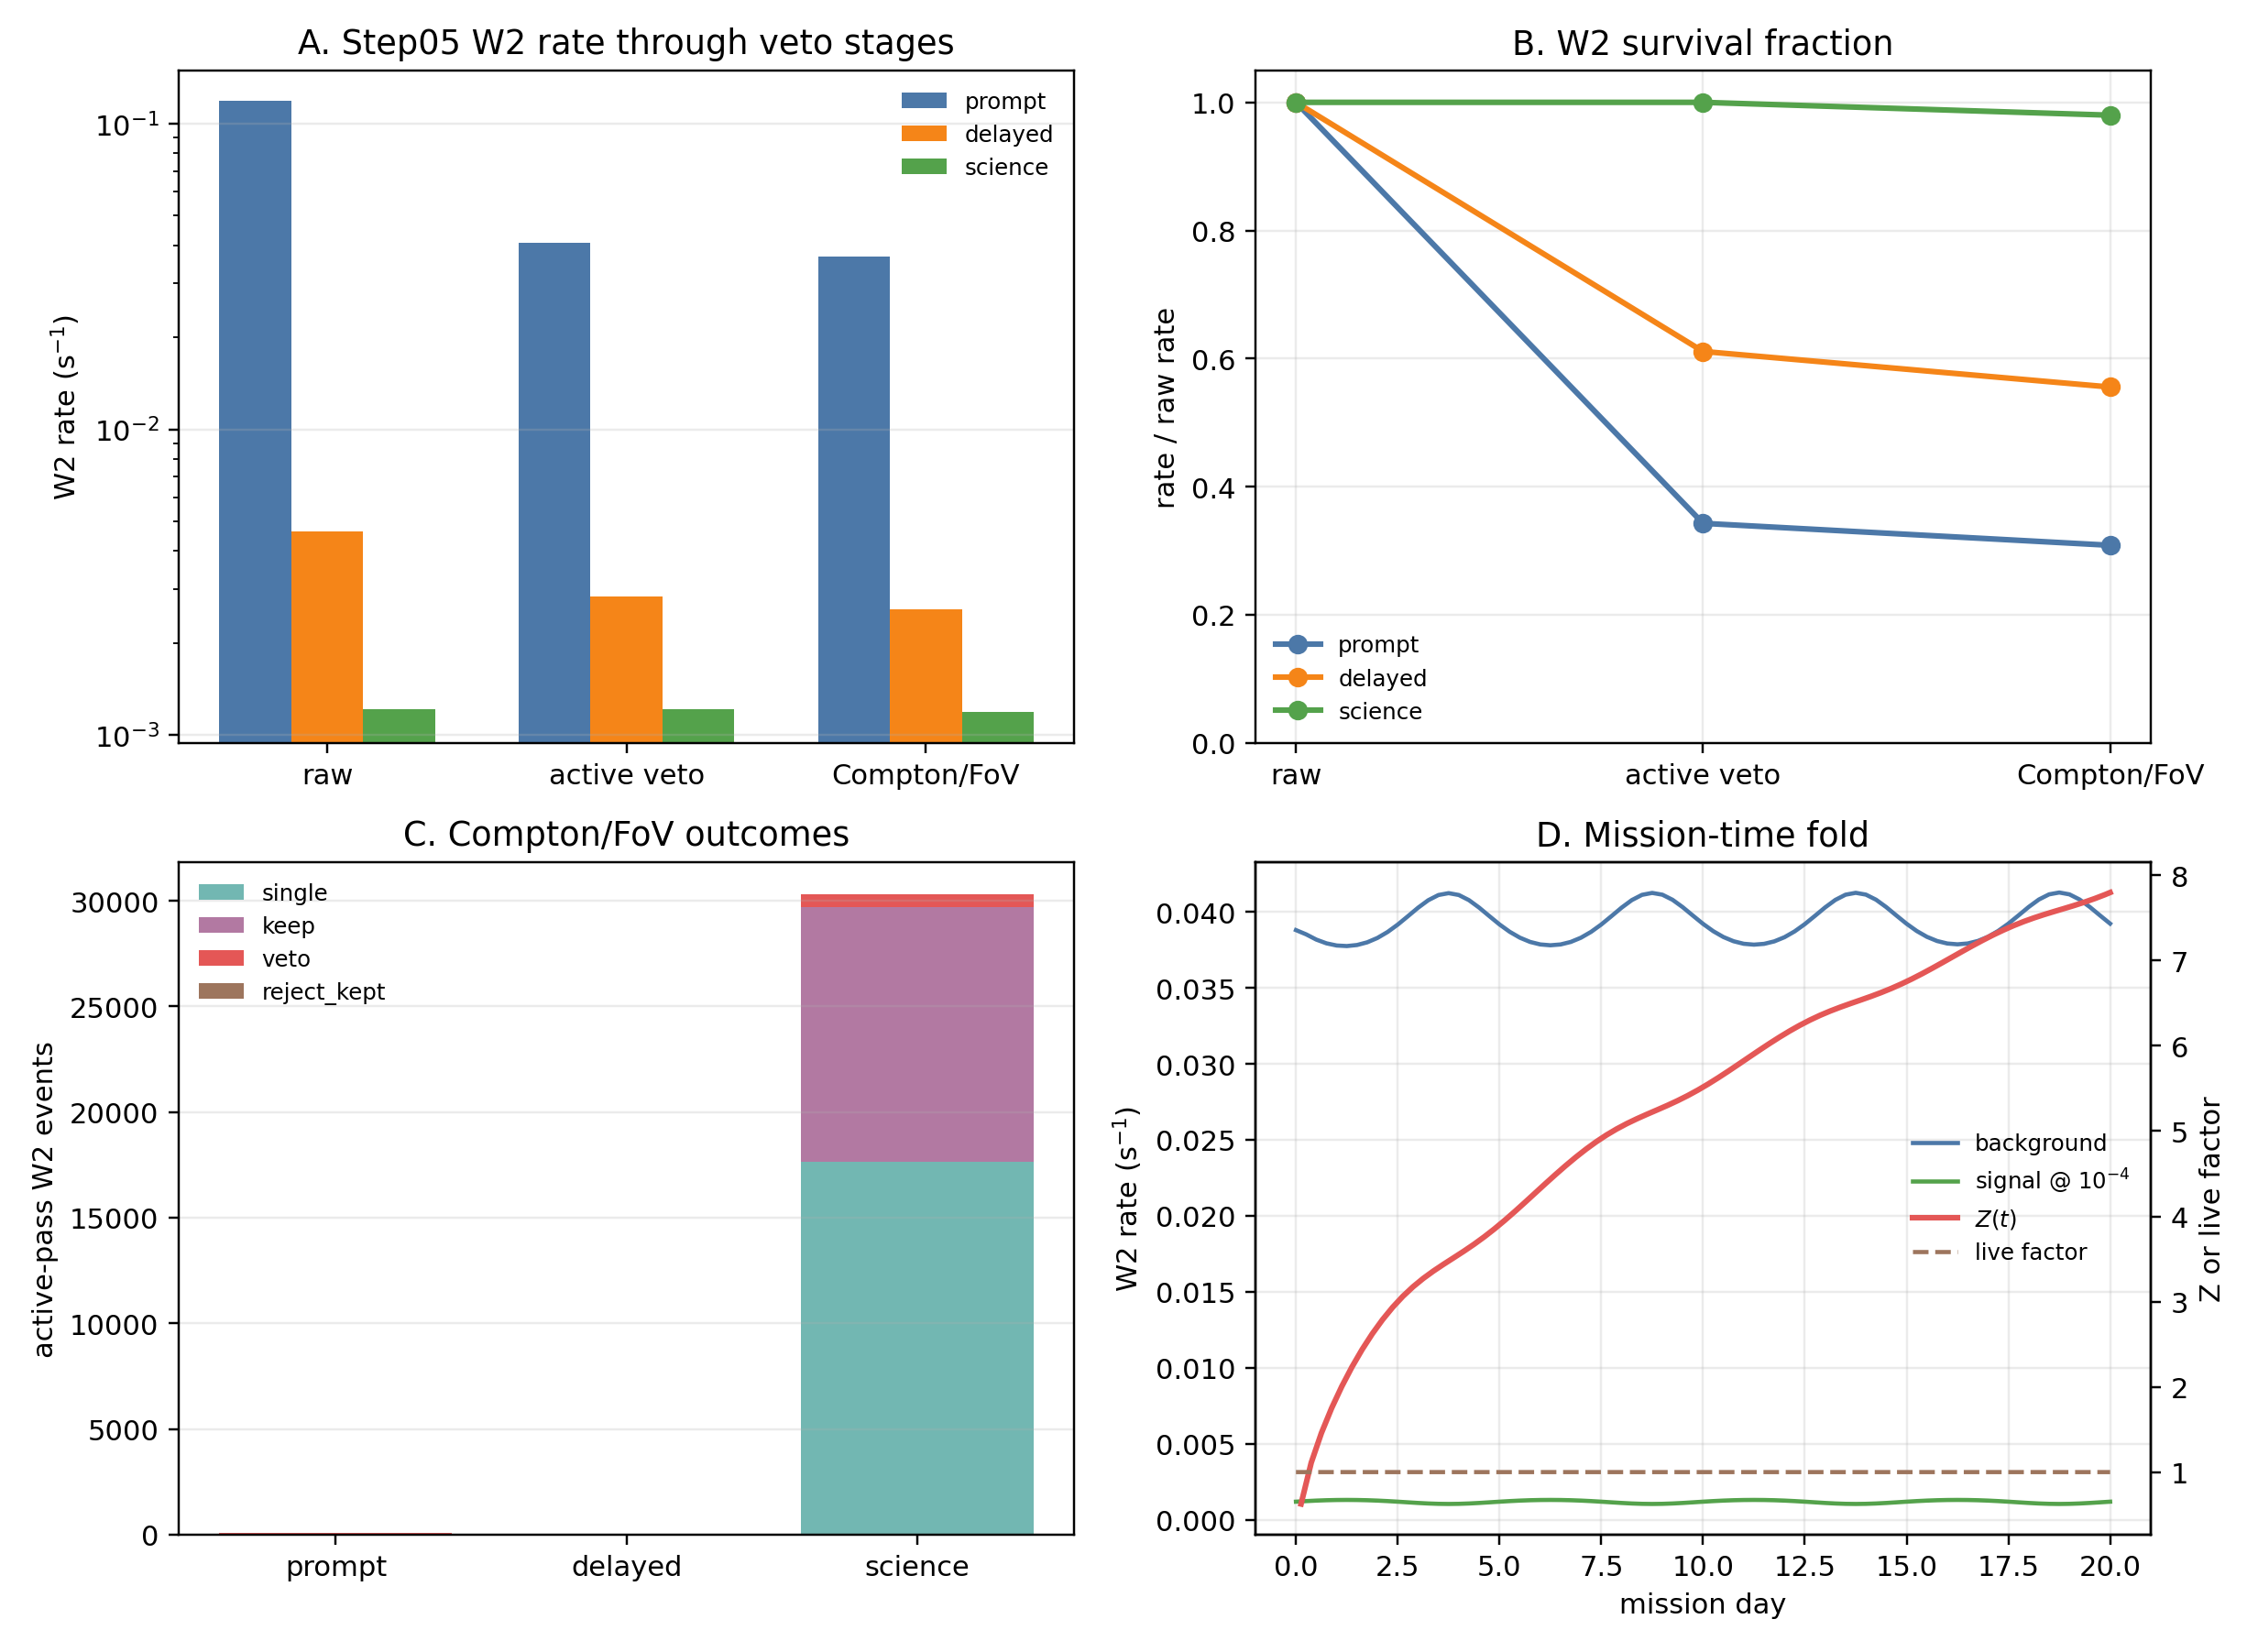
\includegraphics[width=\linewidth]{paper_source_figure_table/fig_selection_veto_time_axis.png}
\caption{当前 fix5 $M=50000$ 精确位置延迟源链路的探测器选择和任务时间折叠诊断。
A 面板给出 $\wii$ 中瞬发本底、延迟活化以及按 $\fzero=10^{-4}\cms$
缩放的聚焦信号在未筛选、主动屏蔽通过和 Compton/FoV 通过三个阶段的率。
B 面板给出相应保留比例。C 面板给出主动屏蔽通过后 Compton/FoV
分类。D 面板给出参考点源情形的任务时间率折叠，并显示解析
偶然符合活时间因子。}
\label{fig:selection_time_axis}
\end{figure}

\begin{figure}[t]
\centering
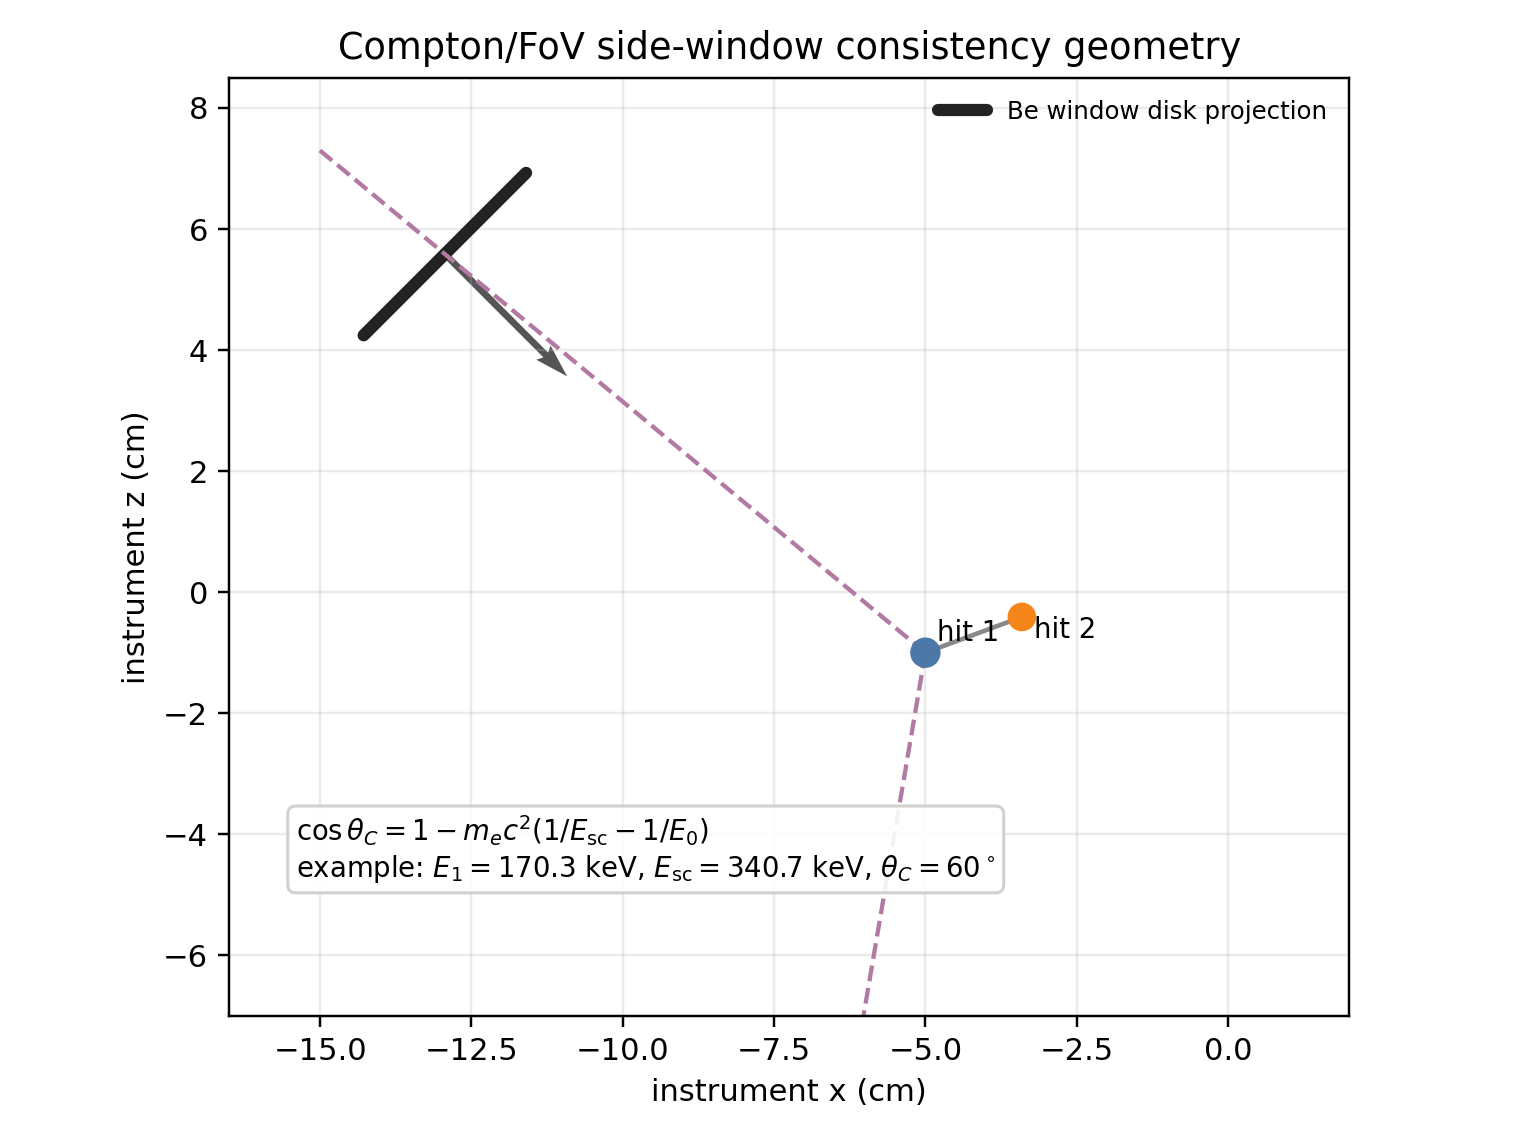
\includegraphics[width=0.78\linewidth]{paper_source_figure_table/fig_compton_fov_geometry.png}
\caption{康普顿/视场一致性检验所用几何。Be 窗圆盘投影由探测器坐标定义
使用的侧入射窗口中心、法向和半径生成。双命中和更高多重度候选
通过测试第一散射康普顿锥是否与该孔径相交来判定，而不是要求其与某个
拟合聚焦光斑一致。}
\label{fig:compton_fov_geometry}
\end{figure}

\section{任务时间轨迹折叠与显著度计算}
\label{sec:mission_time}

探测器选择固定之后，第 15 天选后率沿一个参考任务时间轨迹折叠。这一层
是率级修正：不会在每个任务时间点重新运行 Geant4/MEGAlib 输运。时间
网格包含从 0 到 20 d 的 81 个点，间隔 0.25 d；端点在计数积分中取半宽。
该轨迹是合成参考曲线，不是气球遥测。对以天为单位的时间点 $t_i$，
\begin{align}
  h_i &= h_0+\Delta h\sin\!\left[\frac{2\pi(t_i-15)}{5}\right],\\
  \varphi_i &= \varphi_0+\Delta\varphi\sin\!\left[\frac{2\pi(t_i-15)}{7}\right],\\
  \ell_i &= \ell_0+\Delta\ell\sin\!\left[\frac{2\pi(t_i-15)}{9}\right],
\end{align}
其中 $h_0=38.75\,\mathrm{km}$、$\Delta h=2.5\,\mathrm{km}$、
$\varphi_0=34^\circ$、$\Delta\varphi=0.25^\circ$、$\ell_0=100^\circ$、
$\Delta\ell=0.25^\circ$。由此得到的海拔范围为
$36.25$--$41.25\,\mathrm{km}$，纬度范围为 $33.75^\circ$--$34.25^\circ$，
经度范围为 $99.75^\circ$--$100.25^\circ$。

大气深度和 511 keV 透过缩放写为
\begin{align}
  X(h_i) &= X_{38}\exp\!\left[-\frac{h_i-38\,\mathrm{km}}{H}\right],
       & X_{38}&=3.86510\,\mathrm{g\,cm^{-2}},\quad H=6.8\,\mathrm{km},\\
  T_i &= \exp[-\mu_{\mathrm{eff}} X(h_i)],
       & \mu_{\mathrm{eff}}&=-\frac{\ln T_{15}}{X(h_0)},
\end{align}
其中 $T_{15}=0.7390423888027$。聚焦科学信号的大气缩放为
$f_{\mathrm{atm},i}=T_i/T_{15}$。瞬发大气源缩放为
\begin{align}
  R_{c,i} &= 11.0 -0.08(\varphi_i-\varphi_0)+0.03(\ell_i-\ell_0),\\
  f_{\mathrm{p},i} &=
  \exp\!\left[\frac{X(h_i)-X(h_0)}{30\,\mathrm{g\,cm^{-2}}}\right]
  \left(\frac{11.0}{R_{c,i}}\right)^{0.2}.
\end{align}
延迟活化在求解各核素半衰期演化之前使用同一个标量产生率驱动。对衰变
常数为 $\lambda_a$、固定第 15 天活度为 $A_{a,15}$ 的一个延迟产生元素
$a$，
\begin{align}
  P_{a,15} &= \frac{A_{a,15}}{1-\exp(-\lambda_a t_{15})},\\
  \frac{dN_a}{dt} &= P_{a,15}f_{\mathrm{p}}(t)-\lambda_a N_a,\qquad
  A_a(t)=\lambda_a N_a(t).
\end{align}
数值折叠把解在第 15 天重新锚定到 $A_{a,15}$，再对核素、材料和产生位置
元素求和。

该延迟活度处理假设在这一小范围轨迹内，归一化活化产物分布基本不变，
轨迹只改变标量产生率驱动。这里的验证证明的是这个模型的公式和记账闭合，
而不是证明不同海拔、经纬度下的产生分布在物理上必然不变。如果在轨迹
中心和极值点的专门活化输运显示材料或核素分布发生重分配，则应把标量
驱动替换为产生向量插值：
\begin{equation}
  P_a(t_i)=\sum_g w_g(h_i,\varphi_i,\ell_i,R_{c,i})P_a^{(g)},\qquad
  \sum_g w_g=1,
\end{equation}
然后求解同一组衰变 ODE。

轻量验证在中心点和两个海拔极值点重新计算了轨迹公式。第 15 天中心点
为 $h=38.75\,\mathrm{km}$、$T=0.739042388803$、$f_{\mathrm{p}}=1$，
延迟活度缩放为 1。高海拔探针在第 1.25 天，$h=41.25\,\mathrm{km}$、
$T=0.811094979198$、$f_{\mathrm{p}}=0.965181809612$，延迟活度缩放为
0.913070839359。低海拔探针在第 3.75 天，$h=36.25\,\mathrm{km}$、
$T=0.646122572391$、$f_{\mathrm{p}}=1.05298763053$，延迟活度缩放为
1.02178977033。这些探针处的最大公式偏差为零。用第 15 天率和这些缩放
重构 $\wii$ 瞬发、延迟、本底和信号率也给出零相对偏差，最终累计信号
计数、本底计数和 $Z_{20\mathrm{d}}$ 与显著度摘要值完全一致。

第二个烟测检验该近似的物理部分，但只检验到入射粒子族重混合这一层。
我们在低海拔、第 15 天中心点和高海拔三个轨迹探针处重新生成本地
PARMA 谱，并把它们与按入射粒子族分组的全统计活化积累同位素库比较。
用 PARMA 粒子族缩放重权重第 15 天核素/体积活度贡献后，归一化核素--体积
活度分布的 total-variation 距离最大为 $5.72\times10^{-3}$。PARMA 粒子族
分布距离最大为 $6.76\times10^{-4}$，粒子能量分箱距离最大为
$9.05\times10^{-3}$；解析产生表中可匹配到基态活度修正的活度占比为
0.9929。这个结果支持在当前小范围轨迹内，把延迟产生率/活度折叠作为
标量缩放用于入射粒子族重权重层面。它不是分布不变性的完整物理证明：
同一粒子种类内部的能量/角度相关活化截面变化和输运位置漂移，仍需要在
低海拔、参考点和高海拔分别运行专门的活化产生输运来直接检验。

在任务时间折叠中，第 15 天选后率按该轨迹网格折叠为
\begin{align}
  B_i &= L_i\left(B_{\mathrm{p},15} f_{\mathrm{p},i}
        + B_{\mathrm{d},15} f_{\mathrm{d},i}\right),\\
  S_i &= L_i S_{15} f_{\mathrm{atm},i},\\
  L_i &= \exp[-(R_{\mathrm{p},i}+R_{\mathrm{d},i})\tau],
\end{align}
其中 $f_{\mathrm{p},i}$ 是瞬发大气缩放，$f_{\mathrm{d},i}$ 是延迟活度
缩放，$f_{\mathrm{atm},i}$ 是 511 keV 大气透过缩放，$L_i$ 是偶然
符合活时间因子。这里 $R_{\mathrm{p},i}$ 和 $R_{\mathrm{d},i}$ 是该任务
时间点进入符合分组的瞬发和延迟事例率。

时间相关显著度采用累积计数统计。对参考流量 $\fzero$，累积显著度为
\begin{equation}
  Z(t_m) = \frac{N_s(t_m)}{\sqrt{N_b(t_m)}},
\end{equation}
其中
\begin{equation}
  N_s(t_m)=\sum_{i\leq m}S_i\Delta t_i,\qquad
  N_b(t_m)=\sum_{i\leq m}B_i\Delta t_i
\end{equation}
分别为经过任务时间缩放和 live-factor 修正后的积分信号计数和本底计数。
用于比较不同分析变体的 $3\sigma$ 流量阈值按
\begin{equation}
  \fthree(t_m) = \fzero \frac{3}{Z(t_m)}
\end{equation}
缩放。硬线窗结果和次级比较均使用这一 Gaussian counting 约定。
对主要 20 d 硬线窗结果，任务折叠后的计数约为
$1.09\times10^5$ 个本底计数和 $2.0\times10^3$ 个 $\fzero$ 信号计数，
因此这一近似只用于高计数选后率情形。上游 Ge 代理分量的零选出事例
结果则单独用 Poisson 零计数上限报告。
探测器选择摘要还记录第 15 天直接期望。本文主要结果不采用该
常率直接值，而使用任务时间折叠和最终累积显著度。
对当前硬线窗而言二者差异不大，但明确区分这两类量是比较不同分析配置
的必要条件。

\section{结果}
\label{sec:results}

\subsection{主要硬线窗灵敏度}
\label{subsec:primary}

表~\ref{tab:primary_sensitivity} 给出主要硬线窗结果。在当前 fix5 精确位置链路中，对 $\fzero=10^{-4}\cms$，第 15 天选后率为
\begin{equation}
  B_{\wii}=0.0392162\cps,\qquad
  S_{\wii}=0.00118587\cps .
\end{equation}
任务时间折叠后，平均选后率为
\begin{equation}
  \bar{B}_{\wii}=0.0393546\cps,\qquad
  \bar{S}_{\wii}=0.00117748\cps .
\end{equation}
对应 20 d 显著度为 $Z_{20\mathrm{d}}=7.79950$，$3\sigma$ 探测时间 $2.50573$ d。20 d $3\sigma$ 流量阈值为 $3.84640\times10^{-5}\cms$。

\begin{table}[t]
\centering
\caption{主要 fix5 灵敏度和上一版权威链比较。fix5 精确位置硬线窗行为主要率级结果；上一版 v3p5 行仅用于说明升级比较，不是第二个当前几何。}
\label{tab:primary_sensitivity}
\footnotesize
\resizebox{\linewidth}{!}{%
\begin{tabular}{llccccc}
\toprule
情形 & 基准链路 & $B_{\wii}$ (cps) & $\fzero$ 下 $S_{\wii}$ (cps) & $Z_{20\mathrm{d}}$ & $T_{3\sigma}$ (d) & $\fthree(20\mathrm{d})$ \\
\midrule
fix5 硬线窗 & fix5 精确位置 & 0.0392162 & 0.00118587 & 7.79950 & 2.50573 & $3.84640\times10^{-5}$ \\
上一版权威链 & v3p5 精确位置 & 0.0629804 & 0.00118117 & 6.13039 & 4.77766 & $4.89365\times10^{-5}$ \\
Step05 常率检查 & fix5 第 15 天直接值 & 0.0392162 & 0.00118587 & 7.87187 & 2.90480 & $3.81104\times10^{-5}$ \\
\bottomrule
\end{tabular}
}
\vspace{0.5ex}
\begin{minipage}{0.94\linewidth}
\footnotesize
Step05 直接值是在任务时间折叠前的常率诊断；升级后的主结果为 fix5
累积时间依赖行。归档的空间和斜程行仍是诊断项，不用于改善硬线窗头条阈值。
\end{minipage}
\end{table}

硬线窗行使用窄能窗、主动屏蔽 veto、拓扑/视场一致性选择和任务时间折叠。上一版权威链行显示 fix5 升级判据中的替代比较：总选后本底降低 37.7\%，信号响应保持在 0.4\% 水平，20 d 流量阈值降低 21.4\%。空间门限、45$^\circ$ 视线折叠和固定模板多环似然仍是归档边界检验和后处理分析，而不是最终包含本底扰动参数剖面化的似然结果。

\subsection{本底组成}
\label{subsec:bgcomp}

fix5 精确位置 $\wii$ 选后本底由瞬发大气事例主导。选后流分解为
\begin{equation}
  B_{\mathrm{prompt}}=0.0366410\cps,\qquad
  B_{\mathrm{delayed}}=0.00257520\cps ,
\end{equation}
对应总选后硬线窗本底的 93.43\% 和 6.57\%。选后 W/准直器来源延迟审计把延迟选后事例反查到采样的精确位置源清单，得到零个 W/准直器来源选后事例。表~\ref{tab:bgcomp} 列出这些选后率成分和 W/准直器活化检查。

\begin{table}[t]
\centering
\caption{当前 fix5 精确位置链路中选后 $\wii$ 本底组成。除特别说明外，百分比相对于总 $\wii$ 本底。}
\label{tab:bgcomp}
\footnotesize
\resizebox{\linewidth}{!}{%
\begin{tabular}{lcc}
\toprule
成分 & 率 (cps) & 比例 \\
\midrule
全部瞬发大气流 & 0.0366410 & 93.43\% \\
全部延迟活化流 & 0.00257520 & 6.57\% \\
W/准直器来源延迟选后事例 & 0 & 延迟选后事例的 0\% \\
W/准直器固定源活度 & $0.986080\,\mathrm{Bq}$ & 固定延迟活度的 1.154\% \\
\bottomrule
\end{tabular}
}
\end{table}

\subsection{fix5 源清单和延迟活化审计}
\label{subsec:convergence}

表~\ref{tab:convergence} 总结当前 fix5 精确位置闭环附带的源清单和选后事例检查。这些检查替代旧 v3p5 M 抽样扫描，作为当前几何的升级证据。旧扫描仍是方法检查，但当前通过/失败判据基于全统计 $M=50000$、随机种子 260613 的 fix5 源、其归一化审计，以及下游选后 W/准直器审计。

固定源包含 251,681 条加权产生位置行和 50,000 个等活度点源块。源文本通量和为 $85.4492025\,\mathrm{Bq}$，相对通量差为 $4.54\times10^{-10}$。NUBASE 基态修正把原始延迟活度从 $87.4833$ 降至 $85.4492\,\mathrm{Bq}$。W/准直器体积含有 $0.986080\,\mathrm{Bq}$ 源级活度，但选后事例审计在 30 个延迟选后事例中找到零个 W/准直器来源事例。

\begin{table}[t]
\centering
\caption{当前 fix5 延迟源清单和选后事例审计。}
\label{tab:convergence}
\resizebox{\linewidth}{!}{%
\begin{tabular}{lllll}
\toprule
检查 & 数值 & 状态 & 范围 & 解释 \\
\midrule
精确位置源块 & $M=50000$，种子 260613 & PASS & 源构建 & 全统计 fix5 延迟源 \\
加权源清单 & 251,681 行，$85.449203\,\mathrm{Bq}$ & PASS & 源归一化 & 保活度采样源 \\
源文本通量闭合 & 相对差 $4.54\times10^{-10}$ & PASS & 源序列化 & 源卡归一化无漂移 \\
基态修正 & $87.4833\rightarrow85.4492\,\mathrm{Bq}$ & PASS & 延迟活度 & 已施加 NUBASE 基态半衰期修正 \\
选后 W/准直器审计 & 0 个 W/准直器选后事例 & PASS & 探测器选后延迟事例 & W 活化不是主导选后率成分 \\
\bottomrule
\end{tabular}
}
\end{table}

\subsection{fix5 相对上一版权威链的全统计升级判据}
\label{subsec:fix5_promotion}

表~\ref{tab:bgo_control} 总结全统计升级比较。当前 fix5 硬线窗结果与上一版 v3p5 精确位置权威链使用同一选后率定义比较。旧 new-geometry 的瞬发和延迟总量不作为通过/失败参考，因为基准对齐审计显示该链路与当前选择和源面归一化不能直接比较。

\begin{table}[t]
\centering
\caption{fix5 相对上一版 v3p5 精确位置权威链的全统计升级比较。对本底和流量阈值，比值低于 1 表示改善；对信号保持和显著度，比值高于 1 表示改善。}
\label{tab:bgo_control}
\footnotesize
\resizebox{\linewidth}{!}{%
\begin{tabular}{lccc}
\toprule
指标 & fix5 & 上一版 v3p5 & fix5/v3p5 \\
\midrule
第 15 天总 $B_{\wii}$ (cps) & 0.0392162 & 0.0629804 & 0.6227 \\
延迟 $B_{\wii}$ (cps) & 0.00257520 & 0.00389764 & 0.6607 \\
$\fzero$ 下信号 $S_{\wii}$ (cps) & 0.00118587 & 0.00118117 & 1.0040 \\
累积 $Z_{20\mathrm{d}}$ & 7.79950 & 6.13039 & 1.2723 \\
累积 $\fthree(20\mathrm{d})$ & $3.84640\times10^{-5}$ & $4.89365\times10^{-5}$ & 0.7860 \\
W/准直器来源选后延迟率 & 0 & -- & PASS \\
\bottomrule
\end{tabular}
}
\end{table}

\subsection{上游光学质量代理边界}
\label{subsec:upstream_optics_background}

上游有效 Ge 代理体在第 15 天产生两个隔离的放射性成分，
即 $^{70}$Ga 和 $^{73}$Ga，总活度为 $0.425674\,\mathrm{Bq}$。
使用同一探测器几何和探测器层选择输运 20,000 个延迟衰变后，
$\wii$ 线窗没有选出事例。直接选后率为零，95\% 零计数上限为
$1.25\times10^{-4}\cps$。该上限约为当前 fix5 精确位置 $\wii$ 本底率
$0.0392162\cps$ 的 $0.32\%$，因此隔离的 Ge 代理延迟分量在当前精度
下不改变本文给出的硬线窗灵敏度。上游硬件的瞬发自本底仍不并入主要
预算，因为组合瞬发模拟同时包含普通探测器/低温系统大气瞬发本底，
需要先做来源隔离或显式扣除。明确晶片支撑结构仍是另一个设计级系统项。

\section{讨论}
\label{sec:discussion}

主要结果是，当前 fix5 硬线窗精确位置链路对所建模的聚焦式 TES 线谱仪给出 $3.85\times10^{-5}\cms$ 的 20 d $3\sigma$ 点源阈值。该阈值没有把聚焦光斑空间分析作为主要结果使用，而是来自光学集中、亚 keV 能窗以及探测器耦合 veto/拓扑选择三者的组合。

该计算应作为指向式、窄线、紧凑源灵敏度估计来和现有 511 keV 仪器比较，而不是作为全天成像预测。INTEGRAL/SPI 和 COSI 提供弥散 511 keV 天图的参照测量 \cite{Siegert2016AA,Kierans2020,Siegert2020COSI,Yoneda2025}。NASA 和 HEASARC 任务页面将 COSI 描述为宽视场 0.2--5 MeV Ge 康普顿望远镜；HEASARC 页面给出 Ge 探测器在 511 keV 处 6.0 keV 的能量分辨率 \cite{NASACOSI,HEASARCCOSI}。本文考虑的 TES Laue 透镜概念与其互补：它以天空覆盖换取集中束流和亚 keV 线窗。因此，相关比较对象是紧凑 511 keV 目标、中心核搜索和已知位置瞬变后随观测。相同的聚焦孔径不能替代完整弥散核球和银盘光度测量，因为它只采样很小的立体角。

精确位置延迟源处理针对的是径向分布压缩中的一个具体近似。虽然在当前链路中延迟活化仅占选后硬线窗本底约 6.57\%，但它具有空间和材料结构。保留采样产生位置可避免人为方位角或径向重分布成为未量化系统误差。当前结果采用已输运的 $M=50000$、随机种子 260613 的 fix5 采样情形，并用固定源清单、源卡通量闭合和选后 W/准直器审计作为延迟归一化检查。

本底组成指出了首先应检验的工程敏感项，而不是已经完成的优化结论。选后硬线窗率仍由瞬发大气流主导，因此屏蔽几何、侧入射准直、焦平面附近材料、拓扑选择和多像素事例重建是当前本底最直接的控制项。延迟活化较小，但集中在可识别核素和体积中；当前 W/准直器审计很重要，因为重设计被动材料增加了钨，但选后率显示没有 W/准直器主导的延迟成分。

选后率结果有四个直接边界。第一，探测器/低温系统模型是工程代理，不是最终飞行 CAD；第二，主动屏蔽的定量拒绝在统一探测器层后处理选择中施加，而不是依赖生产阶段触发/反符合过滤；第三，任务时间计算是率级折叠，不是在每个轨迹时间点重新输运粒子；第四，自定义康普顿/视场 veto 尚不是完整 Revan/Mimrec 重建，且保留重建拒绝类是基准接受策略，而不是灵敏度保守下界。

更一般地，表中 $3\sigma$ 流量阈值是基于当前源场、质量模型和探测器响应假设的统计选后率阈值；它们尚未包含大气通量归一化、活化截面或物理列表选择、材料和几何公差、探测器能量响应、veto 阈值标定或重建效率等系统误差包络。

第~\ref{subsec:upstream_optics_background} 节的上游 Laue 透镜计算应理解为等体积、等质量有效 Ge 代理体的边界计算，而不是最终光学硬件本底预算。它已经对该代理体完成全粒子瞬发输运和活化产生输运；隔离出的 Ge 代理延迟成分在当前输运中选出零个 $\wii$ 事例。瞬发自本底贡献仍未纳入主要探测器本底预算，因为它需要先从普通探测器/低温系统瞬发本底中做来源隔离或显式扣除，且明确透镜支撑结构尚未建模。

$r_{90}$ 和多环似然等空间分析可作为诊断，但尚不是投稿级空间--谱联合剖面似然。第~\ref{subsec:fix5_promotion} 节的升级比较是当前 fix5 闭环与上一版 v3p5 精确位置权威链之间的同选择比较。历史 old new-geometry 的瞬发和延迟总量只作为背景信息报告，因为其基准对齐审计显示它不能与当前选择和源面归一化直接比较。因此，可辩护的替代结论是相对 v3p5 权威链：fix5 降低总选后本底，保持信号响应，提高 $Z_{20\mathrm{d}}$，降低 $\fthree(20\mathrm{d})$，且没有引入 W/准直器延迟红旗。

在该率级研究能够支撑飞行性能声明之前，仍有四类验证需要完成：保留多命中子样本的 Revan/Mimrec 交叉检查；包含明确透镜晶片和支撑硬件的全统计量光学硬件自本底输运；最终低温/DR 几何和探测器响应更新，其中包括 TES 饱和与堆积约束；以及可对本底扰动参数做剖面化处理的空间--谱联合似然。

\section{结论}
\label{sec:conclusions}

本文给出了气球载指向式 511 keV TES Laue 透镜望远镜的探测器耦合本底和灵敏度研究。当前 fix5 链路把 Ge(111) Laue 光学响应与 TES 焦平面质量模型、瞬发大气输运、延迟活化、主动屏蔽 veto、康普顿/视场拓扑选择、任务时间率折叠和计数显著度评估结合起来。在主要 $510.58$--$511.42\keV$ 硬线窗中，第 15 天选后率为 $B\simeq3.92\times10^{-2}\cps$，对 $10^{-4}\cms$ 参考点源有 $S\simeq1.19\times10^{-3}\cps$；任务时间折叠后得到 $Z_{20\mathrm{d}}\simeq7.80$ 和 $\fthree(20\mathrm{d})\simeq3.85\times10^{-5}\cms$。相对上一版 v3p5 权威链，这使选后硬线窗本底降至 0.623，20 d 流量阈值降至 0.786，同时保持信号响应。源清单和选后 W/准直器审计表明延迟归一化已闭合，且 W 活化不是主导的选后率成分。该结果为继续评估聚焦式 TES 谱学作为 511 keV 紧凑源和中心核搜索的互补技术提供了探测器耦合选后率依据，同时指出瞬发大气本底抑制和重建验证是下一阶段的主要验证任务。

\section*{数据与软件可用性}
发表前将通过带版本的公开代码仓库或机构存档提供复现本文表格和图所需
的几何与源定义、随机种子、分析和作图脚本、\LaTeX 源文件以及派生验证
产物。归档将包括用于率级计算、收敛性检查、图件来源追踪和文献核验的
机器可读摘要和人工可读验证报告。完整原始输运输出、压缩 Cosima 事例
文件和大型中间事例列表明显大于论文归档包；它们将作为单独的大数据包
归档，或由生成命令、配置文件、校验和或摘要元数据以及派生验证产物
来闭合。

\begin{thebibliography}{99}

\bibitem{Prantzos2011}
N. Prantzos, C. Boehm, A.M. Bykov, R. Diehl, K. Ferriere, N. Guessoum, P. Jean, J. Knoedlseder, A. Marcowith, I.V. Moskalenko, A. Strong, G. Weidenspointner, The 511 keV emission from positron annihilation in the Galaxy, Rev. Mod. Phys. 83 (2011) 1001--1056, doi:10.1103/RevModPhys.83.1001.

\bibitem{Siegert2016AA}
T. Siegert, R. Diehl, G. Khachatryan, M.G.H. Krause, F. Guglielmetti, J. Greiner, A.W. Strong, X. Zhang, Gamma-ray spectroscopy of positron annihilation in the Milky Way, Astron. Astrophys. 586 (2016) A84, doi:10.1051/0004-6361/201527510.

\bibitem{Yoneda2025}
H. Yoneda, T. Siegert, S. Mittal, Imaging the positron annihilation line with 20 years of INTEGRAL/SPI observations, arXiv:2509.01066, 2025.

\bibitem{Kierans2020}
C.A. Kierans, S.E. Boggs, A. Zoglauer, A.W. Lowell, C. Sleator, J. Beechert, T.J. Brandt, P. Jean, H. Lazar, J. Roberts, T. Siegert, J.A. Tomsick, P. von Ballmoos, Detection of the 511 keV Galactic positron annihilation line with COSI, Astrophys. J. 895 (2020) 44, doi:10.3847/1538-4357/ab89a9.

\bibitem{Siegert2020COSI}
T. Siegert, S.E. Boggs, J.A. Tomsick, A.C. Zoglauer, C.A. Kierans, C.C. Sleator, J. Beechert, T.J. Brandt, P. Jean, H. Lazar, A.W. Lowell, J.M. Roberts, P. von Ballmoos, Imaging the 511 keV positron annihilation sky with COSI, Astrophys. J. 897 (2020) 45, doi:10.3847/1538-4357/ab9607.

\bibitem{Siegert2016V404}
T. Siegert, R. Diehl, J. Greiner, M.G.H. Krause, A.M. Beloborodov, M. Cadolle Bel, F. Guglielmetti, J. Rodriguez, A.W. Strong, X. Zhang, Positron annihilation signatures associated with the outburst of the microquasar V404 Cygni, Nature 531 (2016) 341--343, doi:10.1038/nature16978.

\bibitem{Shirazi2023}
F. Shirazi, E. Gau, M.A. Hossen, D. Becker, D. Schmidt, D. Swetz, D. Bennett, D. Braun, F. Kislat, J. Gard, J. Mates, J. Weber, N.R. Cavero, S. Chun, L. Lisalda, A. West, B. Dev, F. Ferrer, R. Bose, J. Ullom, H. Krawczynski, The 511-CAM Mission: A pointed 511 keV gamma-ray telescope with a focal plane detector made of stacked transition edge sensor microcalorimeter arrays, J. Astron. Telesc. Instrum. Syst. 9 (2023) 024006, doi:10.1117/1.JATIS.9.2.024006.

\bibitem{Barriere2009Laue}
N.M. Barriere, L. Natalucci, N. Abrosimov, P. von Ballmoos, P. Bastie, P. Courtois, M. Jentschel, J. Knodlseder, J. Rousselle, P. Ubertini, Soft gamma-ray optics: new Laue lens design and performance estimates, arXiv:0910.0488, 2009.

\bibitem{Barriere2011LauePrototype}
N.M. Barriere, J.A. Tomsick, S.E. Boggs, A. Lowell, P. von Ballmoos, Developing a second generation Laue lens prototype: high reflectivity crystals and accurate assembly, arXiv:1111.6700, 2011.

\bibitem{Weidenspointner2006MAX}
G. Weidenspointner, C.B. Wunderer, N. Barriere, A. Zoglauer, P. von Ballmoos, Monte Carlo study of detector concepts for the MAX Laue Lens gamma-ray telescope, arXiv:astro-ph/0603152, 2006.

\bibitem{SanchezDelRio2011XOP}
M. Sanchez del Rio, R.J. Dejus, XOP v2.4: recent developments of the x-ray optics software toolkit, Proc. SPIE 8141 (2011) 814115, doi:10.1117/12.893911.

\bibitem{Gottardi2021TESReview}
L. Gottardi, K. Nagayoshi, A review of X-ray microcalorimeters based on superconducting transition edge sensors for astrophysics and particle physics, Applied Sciences 11 (2021) 3793, doi:10.3390/app11093793.

\bibitem{Zhang2022TESGamma}
S. Zhang, J.-K. Xia, T. Sun, et al., Transition edge sensor based detector: from X-ray to gamma-ray, arXiv:2204.00010, 2022.

\bibitem{Gehrels1985}
N. Gehrels, Instrumental background in balloon-borne gamma-ray spectrometers and techniques for its reduction, Nucl. Instrum. Methods Phys. Res. A 239 (1985) 324--349, doi:10.1016/0168-9002(85)90732-6.

\bibitem{Sato2015EXPACS}
T. Sato, Analytical model for estimating terrestrial cosmic ray fluxes nearly anytime and anywhere in the world: extension of PARMA/EXPACS, PLoS ONE 10 (2015) e0144679, doi:10.1371/journal.pone.0144679.

\bibitem{Kondev2021NUBASE}
F.G. Kondev, M. Wang, W.J. Huang, S. Naimi, G. Audi, The NUBASE2020 evaluation of nuclear physics properties, Chinese Phys. C 45 (2021) 030001, doi:10.1088/1674-1137/abddae.

\bibitem{Sturner2003}
S.J. Sturner, C.R. Shrader, G. Weidenspointner, B.J. Teegarden, D. Attie, B. Cordier, R. Diehl, C. Ferguson, P. Jean, A. von Kienlin, P. Paul, F. Sanchez, S. Schanne, P. Sizun, G. Skinner, C.B. Wunderer, Monte Carlo simulations and generation of the SPI response, Astron. Astrophys. 411 (2003) L81--L84, doi:10.1051/0004-6361:20031171.

\bibitem{Agostinelli2003}
S. Agostinelli, J. Allison, K. Amako, et al., Geant4---a simulation toolkit, Nucl. Instrum. Methods Phys. Res. A 506 (2003) 250--303, doi:10.1016/S0168-9002(03)01368-8.

\bibitem{Zoglauer2006}
A. Zoglauer, R. Andritschke, F. Schopper, MEGAlib: The Medium Energy Gamma-ray Astronomy Library, New Astron. Rev. 50 (2006) 629--632, doi:10.1016/j.newar.2006.06.049.

\bibitem{Caputo2017}
R. Caputo, F. Kislat, J. Racusin, on behalf of the AMEGO Team, AMEGO: Simulations of the instrument performance, Proc. 35th International Cosmic Ray Conference, PoS(ICRC2017) 783 (2018), doi:10.22323/1.301.0783.

\bibitem{Karwin2023}
C.M. Karwin, T. Siegert, J. Beechert, J.A. Tomsick, T.A. Porter, M. Negro, C. Kierans, M. Ajello, I. Martinez Castellanos, A. Shih, A. Zoglauer, S.E. Boggs, Probing the Galactic diffuse continuum emission with COSI, arXiv:2310.12206, 2023.

\bibitem{Gallego2025}
S. Gallego, U. Oberlack, J. Lommler, C.M. Karwin, F. Fenu, V. Fioretti, A. Zoglauer, et al., Pre-flight background estimates for COSI, arXiv:2510.25304, 2025.

\bibitem{NASACOSI}
NASA Science, COSI mission page, \url{https://science.nasa.gov/mission/cosi/}, accessed 17 June 2026.

\bibitem{HEASARCCOSI}
NASA HEASARC, Compton Spectrometer and Imager (COSI), \url{https://heasarc.gsfc.nasa.gov/docs/heasarc/missions/cosi.html}, accessed 17 June 2026.

\bibitem{Ciabattoni2025ACS}
A. Ciabattoni, V. Fioretti, J.A. Tomsick, A. Zoglauer, P. Patel, L. Mitchell, A. Bulgarelli, P. Jean, G. Panebianco, N. Parmiggiani, C. Vignali, P. von Ballmoos, E. Wulf, Benchmarking of Geant4 simulations for the COSI anticoincidence system, Experimental Astronomy (2025), doi:10.1007/s10686-025-10019-7.

\end{thebibliography}

\end{document}
